\documentclass[a4paper,12pt]{report} % Foglio a4, font size 12, solo fronte
\usepackage[utf8]{inputenc} % Codifica caratteri
\usepackage[lmargin=2cm,rmargin=2cm,tmargin=2.5cm,bmargin=2cm]{geometry} % Bordi pagina come da formato tesi Unibs
\usepackage{charter} % Text font
\usepackage[titles]{tocloft} % TOC compatta
\usepackage{blkarray, bigstrut, amssymb} % Checkmark e altri simboli
\usepackage{graphicx, wrapfig, lipsum} % Per inserire immagini
\usepackage{float} % Per controllare il posizionamento di immagini e tabelle
\usepackage[bottom]{footmisc} % Footer in fondo alla pagina
\usepackage{subcaption} % Subfigures e subcaptions
\usepackage[section]{placeins} % Force all floats before section end
\usepackage{mathtools}
\usepackage{multirow} % For table cells on multiple rows
\usepackage{tabularray}

% Code blocks
\usepackage{listings}
\lstdefinelanguage{plain}{
    basicstyle=\linespread{1.2}\footnotesize\ttfamily,
    stepnumber=1,
    numbersep=8pt,
    showstringspaces=false,
    breaklines=true,
    frame=lines,
    captionpos=b,
    xleftmargin=2em,
    framexleftmargin=1.5em,
    xrightmargin=2em,
    framexrightmargin=1.5em
}
\lstdefinelanguage{numbered}{
    basicstyle=\linespread{1.2}\normalfont\ttfamily,
    numbers=left,
    numberstyle=\scriptsize,
    stepnumber=1,
    numbersep=8pt,
    showstringspaces=false,
    breaklines=true,
    frame=lines,
    captionpos=b,
    xleftmargin=2em,
    framexleftmargin=1.5em,
    xrightmargin=2em,
    framexrightmargin=1.5em
}
\renewcommand\lstlistingname{Code Sample}
\renewcommand\lstlistlistingname{List of Code Samples}
\let\Chapter\chapter
\def\chapter{\addtocontents{lol}{\protect\addvspace{10pt}}\Chapter}

% Glossary
\usepackage[acronym,nonumberlist]{glossaries}
\makeglossaries

% URL
\usepackage[hidelinks]{hyperref} % Per inserire URL
\usepackage{xurl} % Per spezzare URL a capo

% Liste
\usepackage{enumitem} % Per inserire liste
\usepackage{siunitx} % Per usare \setitemize
\setitemize{noitemsep,topsep=0pt,parsep=0pt,partopsep=0pt} % itemize più compatto
\setenumerate{noitemsep,topsep=0pt,parsep=0pt,partopsep=0pt} % enumerate più compatto

% Captions
\usepackage[font=small,textformat=period]{caption}
\captionsetup{justification=centering}

% Numerazione enumerate innestati
\renewcommand{\labelenumii}{\theenumii}
\renewcommand{\theenumii}{\theenumi.\arabic{enumii}.}

% Bibliografia
\usepackage[backend=biber, style=apa]{biblatex} % Bibliografia su un file a parte
\addbibresource{refs.bib} % File contentente la bibliografia

% Spaziature
\linespread{1.5} % Interlinea
\setlength{\parindent}{0pt} % No spazio prima dei paragrafi
\setlength{\parskip}{1em} % Spazio tra paragrafi
\setlength{\headheight}{15pt} % Risolve warning con fancyhdr

% Formato capitoli
\usepackage{titlesec}
\titleformat{\chapter}[hang]{\normalfont\Huge\bfseries}{\thechapter.}{8pt}{\Huge\bfseries}
\titleformat*{\section}{\LARGE\bfseries}
\titleformat*{\subsection}{\Large\bfseries}
\titleformat*{\subsubsection}{\large\bfseries}
\titlespacing*{\chapter}{0pt}{-40pt}{5pt}
\titlespacing*{\section}{0pt}{0pt}{0pt}
\titlespacing*{\subsection}{0pt}{0pt}{0pt}
\titlespacing*{\subsection}{0pt}{0pt}{0pt}
\titlespacing*{\subsubsection}{0pt}{2pt}{0pt}

% Intestazione pagine
\usepackage{fancyhdr}
\pagestyle{fancy}
\renewcommand{\chaptermark}[1]{\markboth{#1}{#1}}
\fancyhf{}
\fancyhead[L]{\nouppercase \leftmark}
\fancyfoot[C]{\thepage}

% Info documento
\title{Study and Development of a Digital Twin for the Simulation of User-Created Automations in a Green Smart Home}
\author{Luca Cotti}
\date{October 2023}

\newacronym{redd}{REDD}{Reference Energy Disaggregation Data Set}
\newacronym{hes}{HES}{Household Electrical Survey}
\newacronym{ihepcds}{IHEPCDS}{Individual Household Electric Power Consumption Data Set}
\newacronym{ampds2}{AMPds2}{Almanac of Minutely Power Dataset Version 2}
\newacronym{eeud}{EEUD}{Electrical-End-Use Dataset}
\newacronym{embed}{EMBED}{Energy Monitoring through Building Electricity Disaggregation}
\newacronym{plaid}{PLAID}{Plug-Load Appliance Identification Dataset}
\newacronym{deddiag}{DEDDIAG}{Domestic Electricity Demand Dataset of Individual Appliances in Germany}
\newacronym{nilm}{NILM}{Non-Intrusive Load Monitoring}
\newacronym{adl}{ADL}{Activities of Daily Living}
\newacronym{ml}{ML}{Machine Learning}
\newacronym{dt}{DT}{Digital Twin}
\newacronym{ac}{AC}{Air Conditioning}
\newacronym{lstm}{LSTM}{Long Short-Term Memory}
\newacronym{bilstm}{BiLSTM}{Bidirectional Long Short-Term Memory}
\newacronym{rnn}{RNN}{Recurrent Neural Network}
\newacronym{relu}{ReLU}{Rectified Linear Unit}
\newacronym{adam}{ADAM}{Adaptive Moment Estimation}
\newacronym{milp}{MILP}{Mixed Integer Linear Programming}
\newacronym{ai}{AI}{Artificial Intelligence}
\newacronym{plm}{PLM}{Product Lifecycle Management}
\newacronym{adt}{ADT}{Airframe Digital Twin}
\newacronym{ct}{CT}{Computer Tomography}
\newacronym{iot}{IoT}{Internet of Things}
\newacronym{eud}{EUD}{End-User Development}

\begin{document}
    \begin{titlepage}
    \begin{figure}[H] % Logo Unibs
        \centering
        
\includegraphics[width=72.4mm]{images/logo_unibs}
    \end{figure}
    
    \begin{center}
        \Large{\uppercase{Dipartimento di Ingegneria dell'Informazione}}\\
        \vspace{4mm}
        \large{Corso di Laurea Magistrale\\
        in Ingegneria Informatica}
    \end{center}

    \vspace{6mm}

    \begin{center}
        \LARGE{\textbf{Study and Development of a Digital Twin for the\\
        Simulation of User-Created Automations\\
        in a Green Smart Home}}\\
    \end{center}

    \vspace{8mm}
    
    \begin{flushleft}
        \large
        \begin{tabular}{ll}
            \large\textbf{Relatrice:} & Prof.ssa Barbara Rita Barricelli\\
            \large\textbf{Correlatrice:} & Chiar.ma Prof.ssa Daniela Fogli \\
        \end{tabular}
    \end{flushleft}

    \vspace{2mm}
    
    \begin{flushright}
        \large
        \textbf{Laureando:}\\
        Luca Cotti\\
        Matricola n. 719204\\
    \end{flushright}

    \vspace*{\fill} % Spazio bianco per mettere il testo in fondo alla pagina

    \centering{\rule{0.6\textwidth}{0.6pt}}\\ % Linea nera
    \centering{\large{Anno Accademico 2022/2023}}
\end{titlepage} % Frontespizio
    \hyphenpenalty=2000 % Meno probabile lo spezzamento delle parole a capo

    \pagenumbering{Roman}
    \tableofcontents
    \printglossary[type=\acronymtype,title=List of Acronyms, nogroupskip]
    \listoffigures
    \listoftables
    \lstlistoflistings

    \cleardoublepage
    \pagenumbering{arabic}
    \chapter{Introduction}\label{ch:introduction}

\begin{itemize}
    \item Motivation and objectives of this thesis
    \item Example of possible uses of the digital twin 
    \item Structure of the thesis 
\end{itemize}
    \chapter{Background}\label{ch:background}

\section{Digital Twins}

A \acrfull{dt} is a physical and/or virtual machines or computer-based model that simulate, emulate, mirror, or ``twin'' the life of a physical entity, which may be an object, a process, a human, or a human-related feature \parencite{barricelliMultiModalApproachCreating2022}. The \acrshort{dt} is linked to its physical counterpart by a bijective relationship.

\begin{itemize}
    \item Definition of digital twin
    \item History of digital twins
    \item Characteristics of digital twins
    \item Opportunities and challenges of digital twins
    \item Digital twins for sustainability
\end{itemize}

\section{Virtual Assistants}

\begin{itemize}
    \item Definition of virtual assistant
    \item IoT ecosystems
    \item Routines
\end{itemize}
    \chapter{Analysis of Smart Home Datasets}\label{ch:analysis_of_smart_home_datasets}

To analyze the smart home datasets available in the literature, a scoping review process based on the procedural steps outlined in \parencite{makStepsConductingScoping2022} was adopted. Three research questions were identified to guide this research:
\begin{enumerate}[label={RQ\arabic*.}, leftmargin=3.5em]
    \item What datasets about appliances are available in the field of smart homes?
    \item Which dataset type is most pertinent to the objectives of this thesis?
    \item What are the characteristics of the datasets falling under the selected type?
\end{enumerate}

The search for relevant literature and datasets initiated from \parencite{barkerSmartOpenData2012}, employing forward snowballing to identify related peer-reviewed publications discussing datasets pertinent to the smart home domain. Additional searches were conducted on Google Scholar, IEEE XPlore, and the Discovery Service of the University of Brescia, utilizing the following search string: \textit{((``Smart Home'' OR ``Home Digital Twin'') AND (``Dataset'' OR ``Data Set''))}. No specific time range was imposed. The search on each engine concluded after two pages with no relevant results. Duplicate entries and non-English results were excluded. Papers about datasets related to the Smart Home subject, or at least mentioned any such dataset, were included. Backward snowballing was subsequently performed on each identified relevant paper. The resulting set of papers was analyzed in order to answer the research questions.

From the compiled list of datasets, only those meeting the following criteria were studied:
\begin{itemize}
    \item The data must originate from actual residential buildings, excluding commercial buildings or laboratory settings.
    \item The dataset must be publicly accessible.
    \item The dataset must include data about household appliances.
    \item Only datasets are considered, not tools for generating datasets.
    \item The study duration must be a minimum of one year, or the dataset should encompass details on at least 15 different appliance types.
\end{itemize}

\newpage

\section{Taxonomy of Smart Home Datasets}

To address RQ1, two types of datasets related to the Smart Home subject that adhere to the criteria outlined above have been identified:
\begin{itemize}
    \item \textit{\acrfull{adl}} datasets, which contain data about the actions of building occupants. Datasets of these type usually gather data from captured images or videos, environmental sensors, devices worn by occupants, or appliance usage.
    \item \textit{Power Consumption} datasets, that encompass data about the energy use in buildings. In the literature, two main groups of power consumption datasets can be identified: appliance-level and aggregated-level. The former traces power consumption of individual devices in buildings, while the latter provides the power consumption of households as a whole.
\end{itemize}
From the above descriptions, it is clear that the datasets of utmost interest for this thesis, addressing RQ2, are power consumption datasets. In particular datasets that contain appliance-level data are the most appropriate. \acrshort{adl} datasets are not relevant for the objectives of this thesis, and as such for remained of this chapter only power consumption datasets will be considered.

\begin{figure}[h]
    \centering
    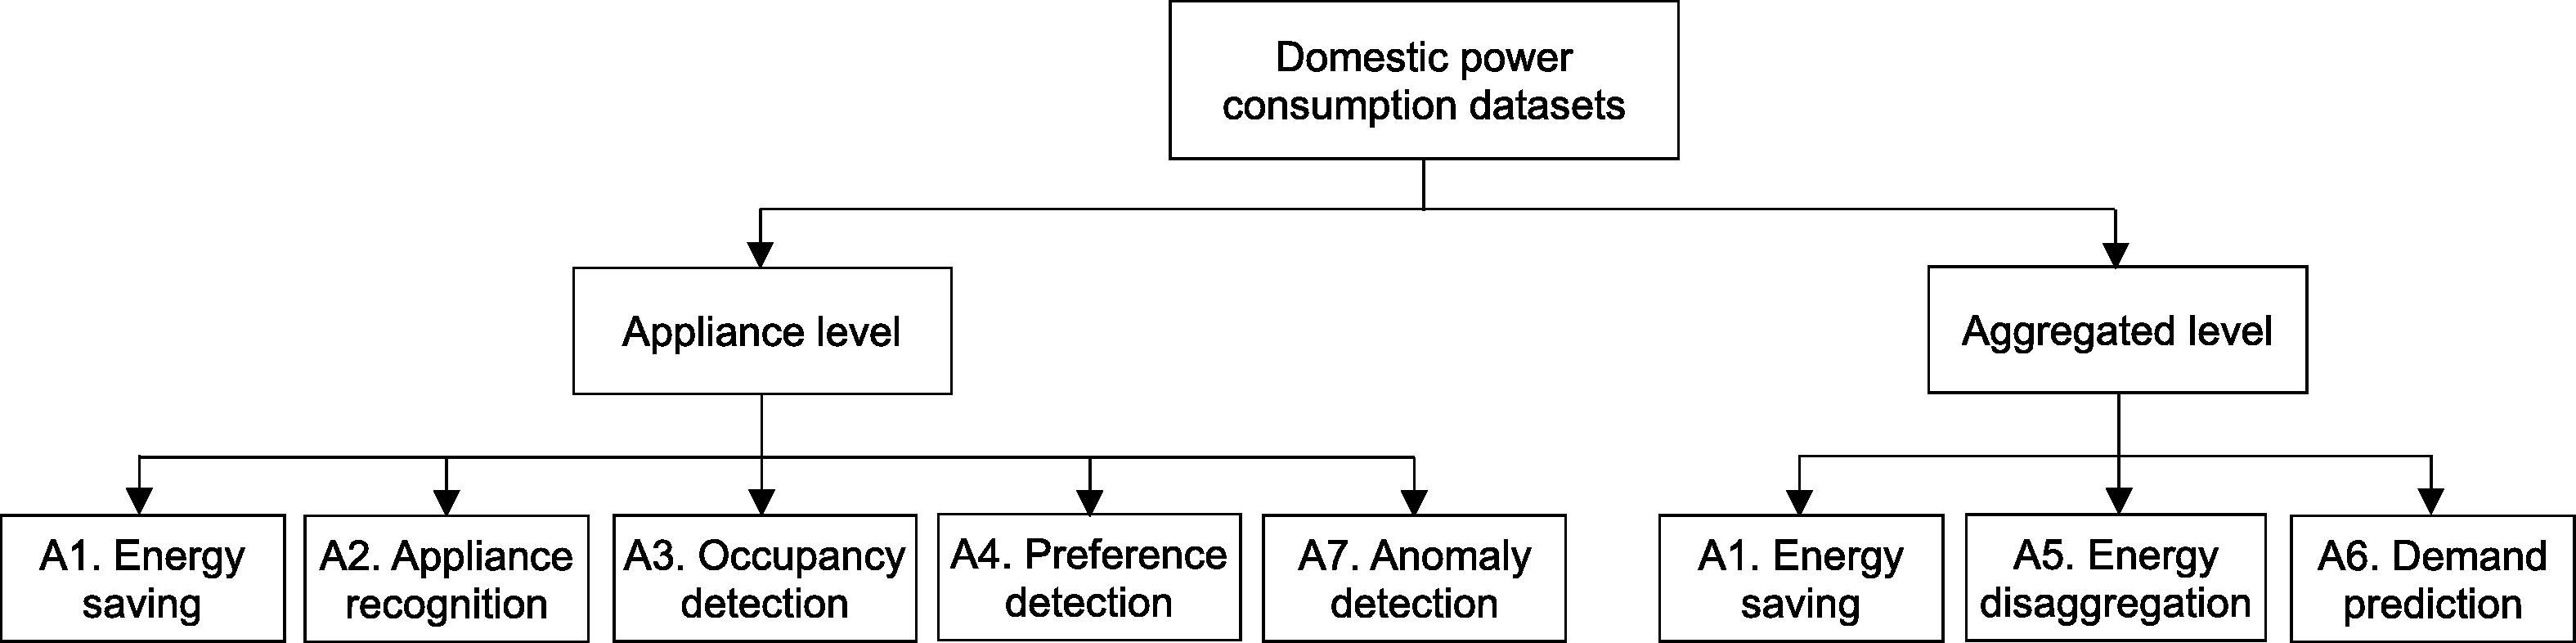
\includegraphics[width=.9\textwidth]{images/taxonomy_power_consumption.jpg}
    \caption[Applications of power consumption datasets]{Applications of power consumption datasets. From~\cite{himeurBuildingPowerConsumption2020}, page 5. CC-BY 4.0 license.}
    \label{fig:applications_power_consumption_datasets}
\end{figure}

In~\parencite{himeurBuildingPowerConsumption2020}, various applications for power consumption datasets are proposed, of which a comprehensive overview illustrated in Figure~\ref{fig:applications_power_consumption_datasets}. It is worth noting that these applications are not mutually exclusive, and as such a single dataset may be appropriate for a number of uses. Application A7 (Anomaly Detection) is out of scope for this thesis, and no dataset for this application will be analyzed.

\newpage

\begin{enumerate}[label={\textit{A\arabic*.}}, leftmargin=3.5em]
    \item \textit{Energy Saving}. Investigating energy-saving measures in buildings can help reduce bills and lower carbon emissions, e.g. by deriving specific recommendations using \acrfull{ml} techniques in order to promote energy efficiency behaviors. Energy saving applications require the dataset to include data from various sources, including energy sub-meters, ambient condition sensors and climate sources.

    \item \textit{Appliance Recognition}. Identifying devices' power usage patterns can help in discriminating their operating conditions. This information can be used, for example, to recognize unattended appliances.

    \item \textit{Occupancy Detection}. By analyzing power consumption profiles and environmental factors like temperature and humidity, it is possible to detect individuals' presence in specific building areas. The assessment of occupancy detection requires datasets with either aggregated or disaggregated power draw, along with a description of consumption scenarios. In particular, the presence of user-driven devices is needed to assume presence in the environment~\parencite{monacchiGREENDEnergyConsumption2014}.

    \item \textit{Preference Detection}, Analyzing energy usage profiles helps evaluate the preferences of occupants. \acrshort{ml} techniques interpret habits related to appliance usage of individuals, understanding their consumption priorities or creating contexts that satisfy their well-being. Datasets for preference detection require appliance-level power consumption.

    \item \textit{Energy Disaggregation}. Also named \acrfull{nilm} in the literature, it consists in separating overall power consumption into signals for individual electrical devices. \acrshort{ml} models can be used to learn the particular power consumption patterns of single devices, with the objective of discerning the contribution of single appliances to the total energy use when only the aggregate consumption data is given. Datasets for energy disaggregation need to include both aggregated and appliance-level consumption fingerprints, to compare the results obtained from disaggregation models with individual patterns of devices.

    \item \textit{Demand Prediction}. \acrshort{ml} algorithms can be used to forecast power demand, aiding public authorities, project managers, and homeowners in energy-efficient planning. Directives and mechanisms can be established in advance with a view of reducing load consumption of equipments and appliances inside infrastructures. Energy demand prediction benefits from power consumption data gathered over an extended collection period.

    \item \textit{Anomaly Detection}. Early detection methods can identify failures in devices and anticipate abnormal energy usage values. For anomaly detection, labeled datasets annotating normal and anomaly consumption footprints are needed.
\end{enumerate}

The frequency used for gathering the data can be significant for certain applications: in load disaggregation, a higher frequency allows for extraction of more representative features capturing the transient behavior~\parencite{carriearmelDisaggregationHolyGrail2013}. Geographical location is also significant, as in the USA nominal voltage in circuits is usually $120V$, while European countries commonly work under $230V$~\parencite{internationalelectrotechnicalcommissionWorldPlugs2024}.

The geographic location of the buildings where data is collected can be significant. Firstly, countries vary in their nominal voltages, with most European and some Asian countries setting single-phase nominal voltages in buildings to $230V$, while in the US and Canada, the value is $120V$~\parencite{leeComparisonAnalysisVoltage2017}. A lower nominal voltage implies that the maximum power draw of single appliances is limited. Additionally, factors like the level of development, climate, efficiency standards for appliance, or the stringency of building codes impact consumption patterns \parencite{berardiCrosscountryComparisonBuilding2017}.

\section{Overview of Power Consumption Datasets}

In this section a description of the characteristics power consumption datasets is provided, answering RQ3. An overview of the datasets is reported in Table~\ref{tab:datasets_overview}, while Table~\ref{tab:datasets_applications} compares the datasets in terms of resolution (both aggregate-level and appliance-level), features provided, and possible applications.

\subsection{REDD}

Released in 2011, the \acrlong{redd}\footnote{\url{https://tokhub.github.io/dbecd/links/redd.html}} is the first and most widely used public dataset in the history of energy disaggregation field~\parencite{iqbalCriticalReviewStateoftheart2020}. It includes aggregated and appliance-specific electricity consumption data from six houses in Massachusetts, USA, collected over several months~\parencite{kolterREDDPublicData2011}. Each monitored house provides two types of electricity data: the whole home signal, recorded with high-frequency monitors (15kHz) on both power phases and a voltage monitor on one phase, and 24 individual circuits labeled with appliance categories, recorded at a low frequency (0.5 Hz). Additionally, data of up to 20 plug-level monitors in the home recorded at 1 Hz is available, with a focus on logging electronics devices where multiple devices are grouped to a single circuit. Energy consumption data for the entire home and specific devices is available for one month. Finally \acrshort{redd} includes labels for the data where possible, which enables the use of supervised \acrshort{ml} approaches.

\subsection{HES}

Resulting from a UK government survey on 251 houses conducted between 2010 and 2011, the \acrlong{hes}\footnote{\url{https://www.gov.uk/government/publications/household-electricity-survey--2}} was released in 2012~\parencite{zimmermannHouseholdElectricitySurvey2012}. While 26 houses were monitored for a year, the rest were monitored for periods of one month at intervals throughout the year. \acrshort{hes}'s limitation is its 2-minute sampling frequency, which makes it inadequate for energy disaggregation as it will be difficult to differentiate between individual devices and occurrences \parencite{himeurBuildingPowerConsumption2020}. However, the dataset provides valuable property information for monitored homes, including building nature, size, room number, and occupants.

\subsection{Tracebase}

The Tracebase\footnote{\url{https://github.com/areinhardt/tracebase}} dataset for appliance identification comprises power consumption traces of individual appliances from 15 houses in Germany and Australia~\parencite{reinhardtAccuracyApplianceIdentification2012}. Collected at a one-sample-per-second resolution, the dataset includes data from 43 distinct appliances, with various recordings spanning multiple days and households. The dataset was released in 2012, but the period during which the data was gathered is not known. While the dataset is valuable for energy efficiency applications, it lacks information on device properties, making it unsuitable for appliance recognition, preference detection, or energy disaggregation \parencite{himeurBuildingPowerConsumption2020}.

\subsection{Smart*}

The UMASS Smart* Home Dataset\footnote{\url{https://traces.cs.umass.edu/index.php/smart/smart}}, released in 2017, features non-continuous data from seven houses in Massachusetts, USA, over three years~\parencite{barkerSmartOpenData2012}. The dataset covers various sources, including electricity usage at mains panels, circuits, and plugs. Additionally, it includes data from weather, motion, door, wall switch, and thermostat sensors, along with electricity generation data from solar panels and wind turbines (every 5 seconds). The data was gathered in high-resolution: for electrical loads, real power each second for entire homes and each circuit is available, along with average real power from almost every individual plug load every few seconds. The dataset also captures on/off/dim events from wall switches and provides voltage and frequency measurements on both phases of the home’s split-leg input power.

\subsection{IHEPCDS}

The \acrlong{ihepcds}\footnote{\url{https://archive.ics.uci.edu/dataset/235/individual+household+electric+power+consumption}}~\parencite{georgeshebrailIndividualHouseholdElectric2006}, released in 2013, contains electricity measurements from a single home near Paris, France. Collected at a one-minute sampling rate, the data spans 47 months, from December 2006 to November 2010. The dataset presents various electrical quantities and sub-metering values, including current, voltage, active and reactive power, with different resolution features.

\subsection{GREEND}

The GREEND\footnote{\url{https://www.andreatonello.com/greend-energy-metering-data-set/}}~\parencite{monacchiGREENDEnergyConsumption2014} is a 1 Hz dataset resulting from a measurement campaign in the Carinthia region of Austria and the Friuli-Venezia Giulia region of Italy. The year-long campaign, started in December 2013, monitored nine houses, aiming to observe and model seasonal consumption behavior of inhabitants. The householders were selected in order to promote diversity of scenarios, for instance involving different types of dwellings and consumers. The dataset includes UTC Unix timestamps for eeasurements, allowing matching with contextual data such as weather.

\subsection{UK-DALE}

The UK-DALE dataset~\parencite{kellyUKDALEDatasetDomestic2015}\footnote{\url{https://jack-kelly.com/data/}} captures appliance-level electricity data from five UK houses. The sample rate is 16 kHz for whole-house consumption and 1/6 Hz for individual appliances. Various versions have been released, with the latest in 2017, covering 4.3 years. The houses were provided by MSc or PhD students from Imperial College, London, who chose the appliances to monitor, prioritizing the most energy-consuming ones as recommended by the authors.


\subsection{AMPds2}

The \acrlong{ampds2}\footnote{\url{https://dataverse.harvard.edu/dataset.xhtml?persistentId=doi:10.7910/DVN/FIE0S4}}~\parencite{makoninElectricityWaterNatural2016} captures electricity, water, and natural gas consumption in a single house near Vancouver, Canada, over two years. The dataset provides 11 measurement characteristics for electricity and includes environmental and utility billing data for cost analysis. \acrshort{ampds2} data is pre-cleaned, with algorithmically filled missing data to maintain a continuous frequency of readings (once per minute). Eleven measurement characteristics of electricity for each meter were presented including active, reactive, and apparent power with other essential parameters.

\subsection{EMBED}

The \acrlong{embed}\footnote{\url{http://embed-dataset.org}}~\parencite{jazizadehEMBEDDatasetEnergy2018} dataset includes aggregate power measurements and plug load data of different appliances for three residential units in Los Angeles, USA. Collected over periods of two to four weeks, the dataset comprises raw current and voltage waveforms along with processed power metrics. \acrshort{embed} is suitable for comparing event-based and non-event-based methodologies, providing fully labeled disaggregation data where by separate labels are identified for different transition states for each appliance.

\subsection{PLAID}

The \acrlong{plaid}\footnote{\url{https://doi.org/10.6084/m9.figshare.10084619.v2}}~\parencite{medicoVoltageCurrentMeasurement2020} contains records of electrical voltage and current from domestic appliances collected at a high sampling frequency of 30 kHz. This is the highest resolution frequency used in existing building power consumption datasets when collecting load profiles \parencite{himeurBuildingPowerConsumption2020}. All appliances are monitored individually: they are sub-metered and the data traces captured over a few seconds include the activation of the appliances. \acrshort{plaid} includes 1876 records from 17 appliance types comprising 330 different makes and models, collected at 65 locations in Pittsburgh, Pennsylvania, USA. Additionally, \acrshort{plaid} covers combined operation records (i.e., measurements obtained when multiple appliances were active simultaneously) and, for some appliances, multiple operating modes were monitored. The dataset does not include traces of active and reactive power.

\subsection{SynD}

SynD\footnote{\url{https://doi.org/10.6084/m9.figshare.c.4716179}} \parencite{klemenjakSyntheticEnergyDataset2020} is a synthetic dataset offering 180 days of  power data for 21 household appliances on both aggregate and per-appliance levels. The dataset, at a sampling frequency of 5 Hz, results from a simulation process based on power traces of real household appliances gathered through a measurement campaign in two households in the Carinthia region of Austria. A dataset generator was used with custom appliance models to simulate one household for given input parameters such as sampling rate and duration. The simulated household can be associated with a relaxed lifestyle of a single person or a young couple. SynD is validated against real appliance consumption for a period of forty days. However, it only considers active power, excluding apparent power, current, or voltage values.

\newpage

\subsection{DEDDIAG}

The \acrlong{deddiag}\footnote{\url{https://doi.org/10.6084/m9.figshare.13615073}}~\parencite{wenningerDEDDIAGDomesticElectricity2021} includes recordings of domestic electricity demand of individual appliances from 15 homes in Germany over a period of up to 3.5 years. In particular, it covers 50 appliances at a 1 Hz frequency over periods of 21 to 1351 days. The dataset is designed for automated domestic load-shift applications. Hence, the dataset contains appliances that have the potential for automated load-shifting such as fridges, freezers, dishwashers, dryers and washing machines. One home also includes three-phase mains readings that can be used for disaggregation tasks. Additionally, \acrshort{deddiag} provides ground truth event annotations for 14 appliances, that provide precise start and stop timestamps. There are multiple labels per appliance where possible in order to annotate different modes. It also includes demographic data for each household's residents such as age, absence duration and regularity of absence.

\begin{table}
    \centering
    \resizebox{\textwidth}{!}{%
        \begin{tabular}{lllp{.1\textwidth}lp{.1\textwidth}lp{.14\textwidth}p{.65\textwidth}}
            \hline
            \textbf{\#} & \textbf{Dataset} & \textbf{Year} & \textbf{Location} & \textbf{Type} & \textbf{\# Houses} & \textbf{Period} & \textbf{\# Appliances} & \textbf{Appliances}                                                                                                                                                                                                                                                                                                                                                                                                                                           \\ \hline
            1           & REDD             & 2011          & USA               & Real-world    & 6                  & 119 days        & 19                     & Furnace, outlets, washing machine, fridge, dish washer, lights, duct heater, dryer, microwave, AC, egauge, panel-GFI, tub, kitchen-counter, wine-cellar, garage-door, barn, well, solar                                                                                                                                                                                                                                                                       \\
            2           & HES              & 2011          & UK                & Real-world    & 251                & 1 year          & 13                     & Fridge, washing machine, washing dryer, dish washer, oven, cooker, hob, microwave oven, kettle, lighting, audiovisual site, television, space heating                                                                                                                                                                                                                                                                                                         \\
            3           & Tracebase        & 2012          & Australia         & Real-world    & 15                 & -               & 39                     & DVD player, hifi-amplifier, subwoofer, vacuum cleaner, desk lamp, MacBook, monitor, alarm clock, amplifier, coffeemaker, breadcutter, cdplayer, charger, stove, TV, dishwasher, ethernet Switch, freezer, iron, dryer, oven, PC, laptop, toaster, USB hard drive, USB Hub, video projector, washing machine, water boiler, water fountain, water kettle, lights, play station, printer, projector, refrigerator, remote desktop, router, solar thermal system \\
            4           & Smart*           & 2012          & USA               & Real-world    & 7                  & 3 years         & 19                     & Furnace, outlets, washing machine, fridge, dish washer, lights, duct heater, dryer, microwave, AC, egauge, panel-GFI, tub, kitchen-counter, wine-cellar, garage-door, barn, well, solar                                                                                                                                                                                                                                                                       \\
            5           & IHEPCDS          & 2013          & France            & Real-world    & 1                  & 47 months       & 9                      & Refrigerator, light, electric water heater, AC, dishwasher, oven, microwave, washing machine, tumble-drier                                                                                                                                                                                                                                                                                                                                                    \\
            6           & GREEND           & 2014          & Austria, Italy    & Real-world    & 9                  & 1 year          & 27                     & Coffee machine, washing machine, radio, water kettle, fridge, dishwasher, lamp, TV, vacuum cleaner, microwave, amplifier, lights, NAS, notebook, bread machine, outlets, hair dryer, computer, oven, scanner, printer, hood, toaster, stove, iron, decoder, ADSL modem                                                                                                                                                                                        \\
            7           & UK-DALE          & 2015          & UK                & Real-world    & 5                  & 4.3 years       & 22                     & Fridge freezer, home theatre PC, dish washer, washer dryer, kettle, AC, lamp, boiler,  breadmaker, soldering iron, computer monitor, toaster, television, vacuum cleaner, printer, ethernet switch, immersion heater, laptop computer, microwave, rice cooker, hair dryier, game console                                                                                                                                                                      \\
            8           & AMPds2           & 2016          & Canada            & Real-world    & 1                  & 2 years         & 11                     & Plugs \& lights, clothes dryer, clothes washer, dishwasher, fridge, furnace, garage, heat pump, instant hot Water unit, TV, oven                                                                                                                                                                                                                                                                                                                              \\
            9           & EMBED            & 2018          & USA               & Real-world    & 3                  & 2-4 weeks       & 21                     & Refrigerator, washing machine, central air conditioning (ac), window ac, toaster, kettle, tv, iron, hair dryer, hair iron, lcd monitor, laptop, light, grill, coffee maker, xbox, bathroom fan, water heater, surface tablet, microwave, electric range                                                                                                                                                                                                       \\
            10          & PLAID            & 2018          & USA               & Real-world    & 65                 & 3 months        & 16                     & AC, blender, coffeemaker, Compact Fluorescent Lamp (CFL), fan, fridge, hair dryer, hair iron, heater, bulb, laptop, microwave, soldering iron, vacuum, washing machine, water kettle                                                                                                                                                                                                                                                                          \\
            11          & SynD             & 2020          & Austria           & Synthetic     & 2                  & 180 days        & 21                     & Fridge, Dishwasher, Electric heater, Washing machine, Toaster, Fan, Microwave, Iron, Hot air gun, Router, Coffee machine, TV, Printer, Laptop computer, Lamp, Gaming PC, Pocket Radio, Monitor, Electric oven, Hair dryer, Water kettle                                                                                                                                                                                                                       \\
            12          & DEDDIAG          & 2021          & Germany           & Real-world    & 15                 & 3.5 years       & 8                      & Coffee machine, dish washer, dryer, freezer, office desk, refrigerator, tv, washing machine                                                                                                                                                                                                                                                                                                                                                                   \\ \hline
        \end{tabular}}
    \caption[Overview of power consumption datasets]{Overview of power consumption datasets.}
    \label{tab:datasets_overview}
\end{table}

\begin{table}
    \centering
    \resizebox{\textwidth}{!}{%
        \begin{tabular}{llllll}
            \hline
            \multirow{2}{*}{\#} & \multirow{2}{*}{Dataset} & \multicolumn{2}{l}{Resolution} & \multirow{2}{*}{Features} & \multirow{2}{*}{Applications}                          \\ \cline{3-4} &  & Aggregate & Appliance &  & \\ \hline
            1                   & REDD                     & 15 kHz                         & 0.5 Hz, 1 Hz              & I, V, P                       & A1, A2, A4, A5         \\
            2                   & HES                      & 2 min or 10 min                & 2 min or 10 min           & I, V, P, T                    & A1, A6                 \\
            3                   & Tracebase                & -                              & 1-8s                      & P, Np                         & A1, A6                 \\
            4                   & Smart*                   & 1 Hz                           & 1 Hz                      & I, V, P, f, S                 & A1, A2, A3, A4, A5, A6 \\
            5                   & IHEPCDS                  & 1 min                          & 1 min                     & I, V, P, Q                    & A1, A6                 \\
            6                   & GREEND                   & 1 Hz                           & 1 Hz                      & P                             & A1, A2, A3, A4, A5, A6 \\
            7                   & UK-DALE                  & 16 kHz                         & 1s, 6s                    & I, V, P, Q, S                 & A1, A2, A3, A4, A5, A6 \\
            8                   & AMPds2                   & 1 min                          & 1 min                     & I, V, P, S, f, pf             & A1, A2, A4, A5         \\
            9                   & EMBED                    & 12 kHz                         & 1 Hz                      & I, V, P, Q                    & A1, A2, A4, A5         \\
            10                  & PLAID                    & -                              & 30 kHz                    & I, V                          & A1, A2, A4             \\
            11                  & SynD                     & 5 Hz                           & 5 Hz                      & P                             & A1, A2, A4, A5         \\
            12                  & DEDDIAG                  & 1 Hz                           & 1 Hz                      & P                             & A1, A2, A4, A5, A6     \\ \hline
        \end{tabular}}
    \caption[Comparison of power consumption datasets in terms of features, resolution, and applications]{Comparison of power consumption datasets in terms of features, resolution, and applications. The features reported are current (I), voltage (V), active power (P), reactive power (Q), apparent power (S), normalized power (Np), frequency (f), power factor (pf), and Temperature (T).}
    \label{tab:datasets_applications}
\end{table}
    \chapter{Hypothetical Home}\label{ch:hypothetical_home}

An hypothetical home was designed as a starting point for the creation of the \acrshort{dt}. A number of appliance types were chosen to be introduced into the home, based on their commonality in European households and their availability in the GREEND and UK-DALE datasets. These two datasets were selected among the ones studied (see Chapter~\ref{ch:analysis_of_smart_home_datasets}) because they provide a large number of appliances, and they contain data about European households. This is significant to minimize the geographic variations in appliance usage patterns and to produce results that can be relevant for Italian households. The floor plan of the home is shown in Figure~\ref{fig:home_floor_plan}, showing the location of the following chosen appliances:
\begin{itemize}
  \item a fridge with a combined freezer;
  \item a washing machine;
  \item a dishwasher;
  \item a radio;
  \item two TVs;
  \item a desktop computer;
  \item six lamps;
  \item a microwave;
  \item three \acrshort{ac} splits;
  \item a boiler.
\end{itemize}

\begin{figure}
  \centering
  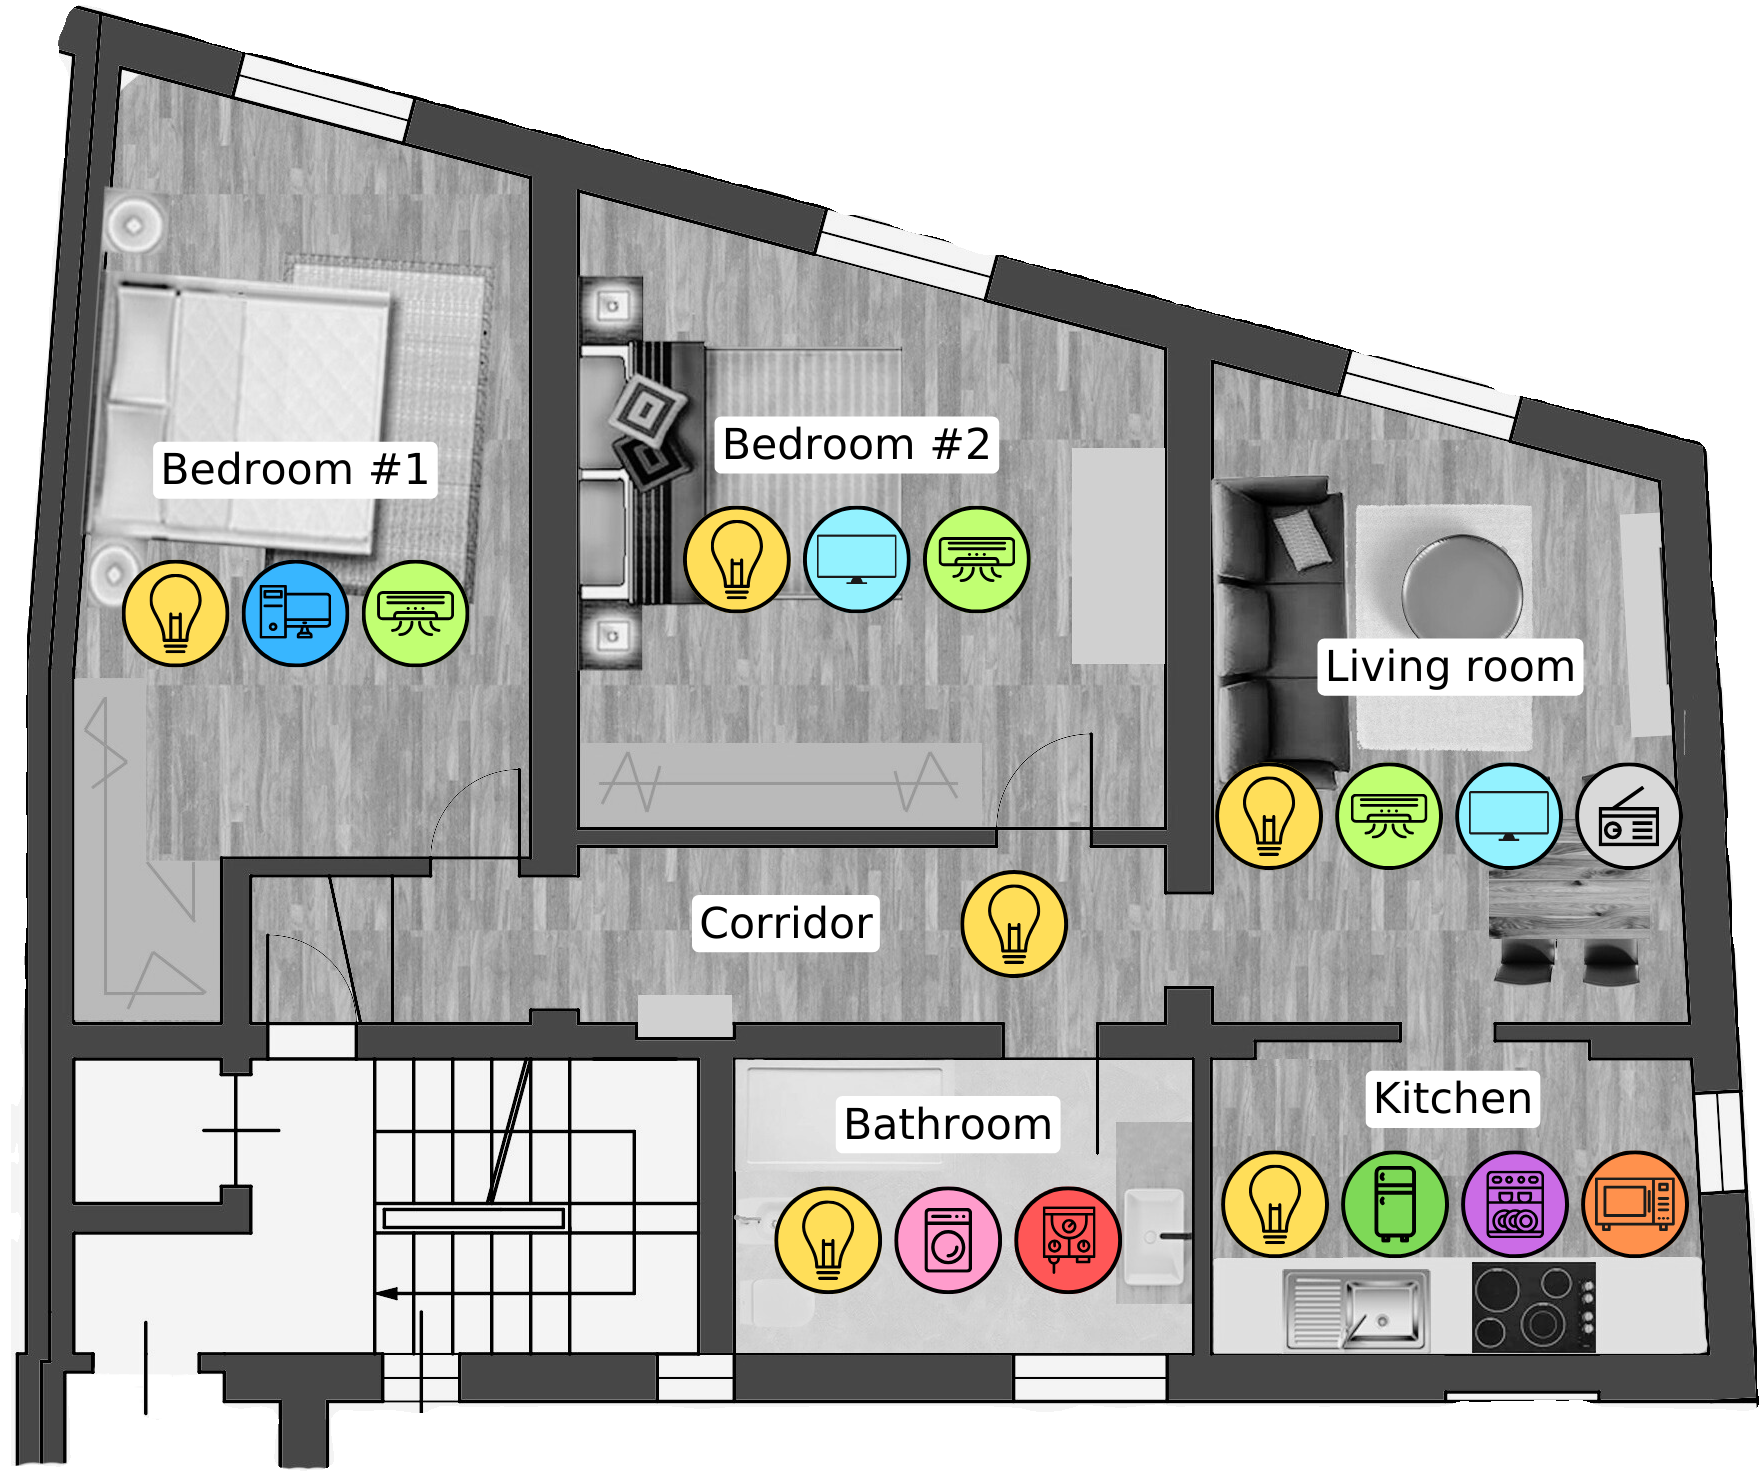
\includegraphics[width=0.75\linewidth]{images/floor_plan.png}
  \caption[Floor plan of a hypothetical case study home with the location of the chosen appliance types.]{Floor plan of a hypothetical case study home with the location of the chosen appliance types. Adapted from the floor plan courtesy of Matteo Pigoli}
  \label{fig:home_floor_plan}
\end{figure}

For each appliance type, a specific appliance studied in one of the buildings in GREEND or UK-DALE was chosen as a representative sample. Table~\ref{tab:appliances_details} shows the details of the selected appliances, including the source dataset, the building, the manufacturer, and the model. The preferred sources were buildings $3$ and $5$ of the GREEND dataset, as they had a large number of appliance data and reasonable consumption values. Other buildings in GREEND were discarded, as they either contained insufficient usage data, or the consumptions were highly unrealistic, indicating measurement errors. The appliance types that were either unavailable or unsuitable in GREEND were instead chosen from the UK-DALE dataset. Again, the buildings and appliances were chosen with the same criteria as GREEND. Because no information about individual \acrshort{ac} splits was available, the whole-home \acrshort{ac} consumption was used instead. This corresponds to the three splits being controlled collectively.

\begin{table}
  \centering
  \begin{tabular}{llcll}
    \hline
    \textbf{Appliance type} & \textbf{Dataset} & \textbf{Building} & \textbf{Manufacturer} & \textbf{Model} \\ \hline
    Radio                   & GREEND           & 3                 & Denon                 & DRA-275RD      \\
    Dishwasher              & GREEND           & 5                 & Whirlpool             & ADG 555 IX     \\
    Fridge w/ freezer       & GREEND           & 5                 & Siemens               &                \\
    Television              & GREEND           & 5                 & Samsung               & LE32C650       \\
    Microwave               & GREEND           & 3                 & Whirlpool             & AMW 494/IX     \\
    Lamp                    & UK-DALE          & 1                 &                       &                \\
    Washing machine         & GREEND           & 3                 & Zanussi               & F1215          \\
    Desktop                 & GREEND           & 5                 & Dimotion              & QuietONE Q2    \\
    Boiler                  & UK-DALE          & 4                 &                       &                \\
    AC                      & UK-DALE          & 5                 &                       &                \\ \hline
  \end{tabular}%
  \caption[Details of selected appliances]{Details of selected appliances. Empty cells indicate that the information is not provided}
  \label{tab:appliances_details}
\end{table}

A limitation of both the GREEND and UK-DALE datasets is that they do not record the operation mode of appliances at a given time. This information is required to assign a specific consumption value to the operation modes and to estimate their duration. The other datasets introduced in Chapter~\ref{ch:analysis_of_smart_home_datasets} that do provide this type of information are either too imprecise about the start/end time or limited in the number of appliances they record.

A possible solution is identifying the operation mode of appliances from the power consumption data using unsupervised learning methods. A naive approach to doing so is clustering the raw energy values: this can work for simple appliances, such as lamps or televisions, but not for complex ones with \textit{operation cycles}, such as fridges or washing machines. For example, a washing machine might draw no power for a short period while the clothes soak, and then use a lot of power for a spin cycle. Both of these cycles are part of the same operation mode, but there is no way to recognize this when clustering the raw data. Furthermore, methods based on raw data are also susceptible to noisy points and outliers; thus, they often lead to poor clustering results~\parencite{castangiaClusteringApplianceOperation2023}.

The approach used in this thesis is inspired by the one proposed by~\textcite{castangiaClusteringApplianceOperation2023}, which uses unsupervised deep learning techniques to cluster appliance operation modes from a learned, \textit{latent state} representation of the raw data. Figure~\ref{fig:high_level_procedure} illustrates the main steps of the approach. First, a segmentation procedure is applied to the raw appliance data to identify the active states that contain the actual power signatures of the device. These signatures are then standardized and fed to a deep autoencoder model, which learns to reconstruct the operation cycles and encode them into a latent representation. Next, a K-means clustering algorithm is applied to the latent representation, which groups the operation cycles into different programs of the device. Finally, the clusters are mapped to the operation modes of the appliance. The remaining sections in this chapter describe the steps in more detail. The code for the extraction of activations is available on GitHub\footnote{\url{https://github.com/LucaCtt/appliances_data_extraction}}, while the remaining steps are executed in a Google Colab notebook\footnote{\url{https://colab.research.google.com/drive/1blnoyyP10gGdRL6b4JzaeBLg8zs2kVv9?usp=sharing}}.

\begin{figure}
  \centering
  
\includegraphics[width=\linewidth]{images/modes_clustering/high_level_procedure.png}
  \caption{High level procedure for identifying the operation modes of appliances}
  \label{fig:high_level_procedure}
\end{figure}

\section{Extraction of Appliances Activations}

An \textit{appliance activation} is defined as a sequence of power consumption values gathered in a time interval in which the appliance is switched on. An example of activation for the fridge in building 3 of GREEND is reported in Listing~\ref{code:activation_example}, which highlights how the consumption values change during the activation. The goal of extracting the activations is to identify the distinct operations of an appliance based on the continuous active power measurements available, which however include time intervals in which the appliances are switched off, and can thus be filtered out. The power consumption when an appliance is off is assumed to be zero.

To identify the activations, the GREEN and UK-DALE datasets were accessed using NILMTK\footnote{\url{https://github.com/nilmtk/nilmtk}}, a Python toolkit designed for comparing the performance of energy disaggregation algorithms~\parencite{batraItDifferentInsights2013}, which also provides data analysis functions for NILM datasets. The appliance activations were extracted at the default frequency of the datasets (every second for GREEND and every six seconds for UK-DALE) using NILMTK's \texttt{Electric.get\_activations()} method, with three arguments used for configuration:
\begin{itemize}
  \item \texttt{on\_power\_threshold}: the minimum power consumption value (in watts) for the appliance to be considered switched on.
  \item \texttt{min\_off\_duration}: the minimum duration (in seconds) for the appliance to be below \texttt{on\_power\_threshold} to be considered turned off.
  \item \texttt{min\_on\_duration}: the minimum duration (in seconds) for the activation to be valid. This, along with \texttt{min\_off\_duration}, helps to filter out spurious power spikes.
\end{itemize}
The values of these parameters were selected empirically for each appliance, by selecting combinations that produced a balance between the number of activations and their mean length. For example, considering the microwave in building 3 of GREEND, using $\texttt{on\_power\_threshold} = 20$, $\texttt{min\_off\_duration} = 20$, and $\texttt{min\_on\_duration} = 10$ resulted in $2311$ activations, with a mean duration of around $471$ seconds. When using instead $\texttt{on\_power\_threshold} = 10$, $\texttt{min\_off\_duration} = 5$, and $\texttt{min\_on\_duration} = 5$ resulted in $15609$ activations, with a mean duration close however to just $78$ seconds.

\newpage

The sampling frequency of the activations is the default one provided by the datasets, which corresponds to $1$ second for GREEND and $6$ seconds UK-DALE. The resulting activations were then clipped to a maximum threshold to eliminate noise. The maximum thresholds were chosen using the plots of the raw power consumption data of each appliance, represented in Figures~\ref{fig:raw_power_consumptions_greend} and~\ref{fig:raw_power_consumptions_uk_dale} using Matplotlib~\parencite{hunterMatplotlib2DGraphics2007}, by selecting values that remove spurious power spikes. It can be observed from Figure~\ref{fig:ac} that the consumptions of the AC are unrealistically high. Due to the lack of other AC appliances in the datasets, the data was clipped and used anyway. Table~\ref{tab:activation_details} shows the parameters and the number of activations obtained for each appliance type.

\begin{lstlisting}[language=plain,caption={[Example of an activation]Example of an activation for the fridge in building 3 of the GREEND dataset. The numbers are samples of the energy consumption (in watts) gathered every second.},label=lst:activation_example,float,floatplacement=H]
0.000000 0.000000 66.601420 120.160070 63.387650 63.387650 173.715010 175.85713 130.871350 10.896457 ... 177.99924 186.56764 186.56764 188.70972 186.56764 201.56210 207.98820 201.56210 207.98820
\end{lstlisting}

\begin{figure}
  \begin{subfigure}{.5\textwidth}
    \centering
    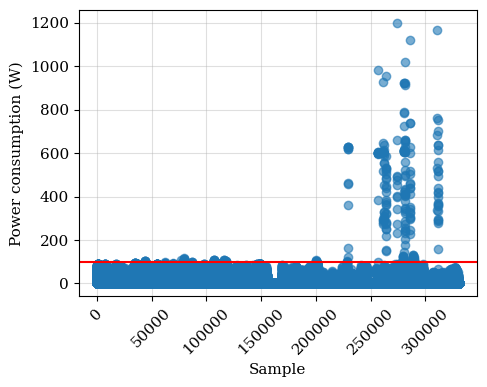
\includegraphics[width=.9\linewidth]{images/raw_consumptions/audio_amplifier.png}
    \caption{Radio}
    \label{fig:radio}
  \end{subfigure}%
  \begin{subfigure}{.5\textwidth}
    \centering
    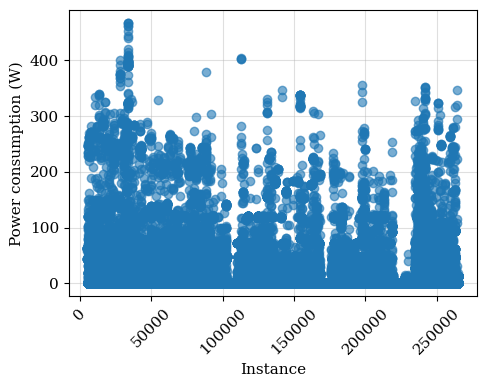
\includegraphics[width=.9\linewidth]{images/raw_consumptions/dish_washer.png}
    \caption{Dishwasher}
    \label{fig:dish_washer}
  \end{subfigure}
  \begin{subfigure}{.5\textwidth}
    \centering
    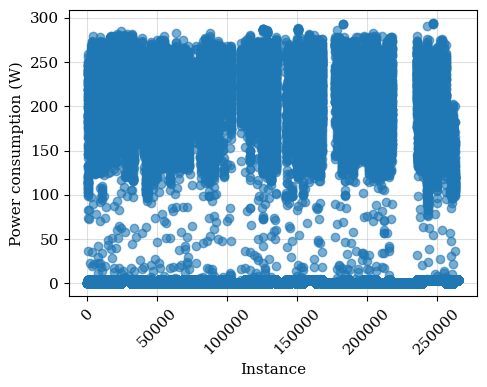
\includegraphics[width=.9\linewidth]{images/raw_consumptions/fridge.png}
    \caption{Fridge freezer}
    \label{fig:fridge_freezer}
  \end{subfigure}%
  \begin{subfigure}{.5\textwidth}
    \centering
    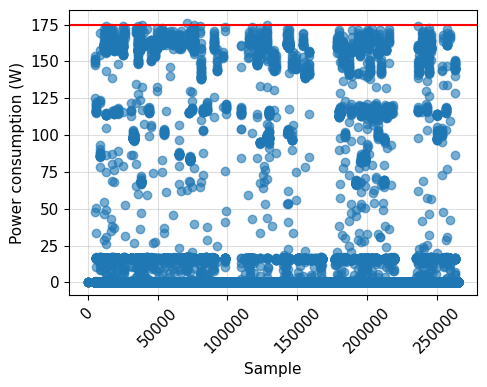
\includegraphics[width=.9\linewidth]{images/raw_consumptions/television.png}
    \caption{Television}
    \label{fig:television}
  \end{subfigure}
  \begin{subfigure}{.5\textwidth}
    \centering
    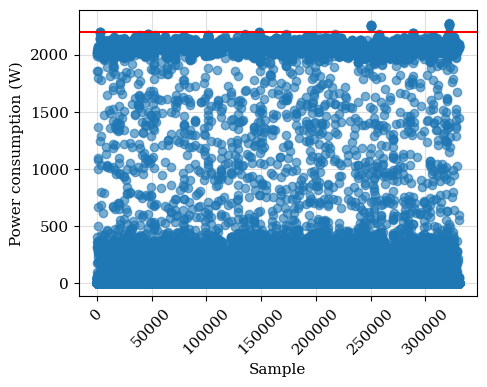
\includegraphics[width=.9\linewidth]{images/raw_consumptions/microwave.png}
    \caption{Microwave}
    \label{fig:microwave}
  \end{subfigure}%
  \begin{subfigure}{.5\textwidth}
    \centering
    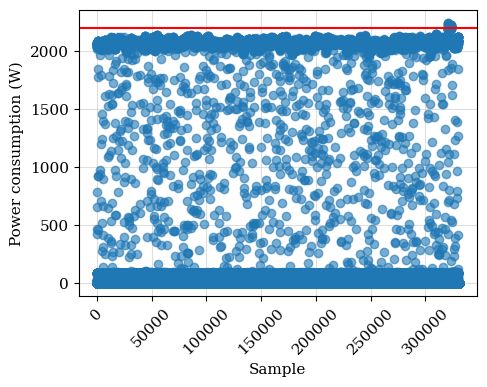
\includegraphics[width=.9\linewidth]{images/raw_consumptions/washing_machine.png}
    \caption{Washing machine}
    \label{fig:washing_machine}
  \end{subfigure}
\end{figure}%
\begin{figure}\ContinuedFloat
  \begin{subfigure}{\textwidth}
    \centering
    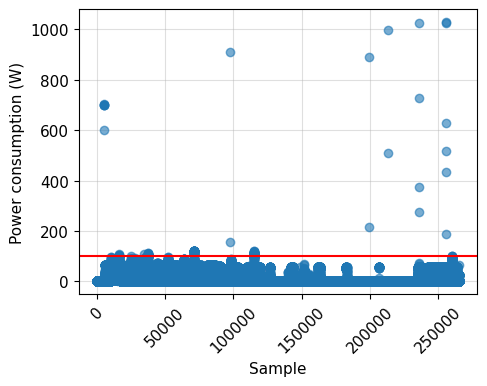
\includegraphics[width=.45\linewidth]{images/raw_consumptions/desktop_computer.png}
    \caption{Desktop computer}
    \label{fig:desktop_computer}
  \end{subfigure}
  \caption[Raw power consumptions of appliances extracted from GREEND]{Raw power consumptions of appliances extracted from GREEND. The samples are gathered every second. The red line represents the maximum threshold used to clip the activations}
  \label{fig:raw_power_consumptions_greend}
\end{figure}

\begin{figure}
  \begin{subfigure}{.5\textwidth}
    \centering
    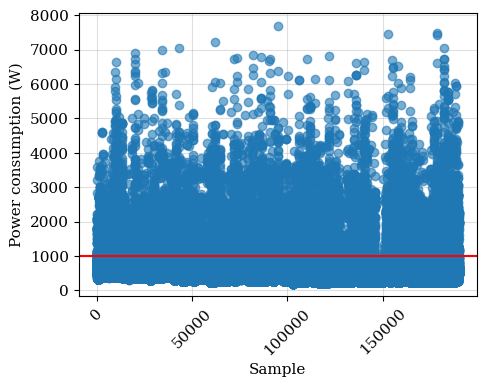
\includegraphics[width=.9\linewidth]{images/raw_consumptions/ac.png}
    \caption{AC}
    \label{fig:ac}
  \end{subfigure}%
  \begin{subfigure}{.5\textwidth}
    \centering
    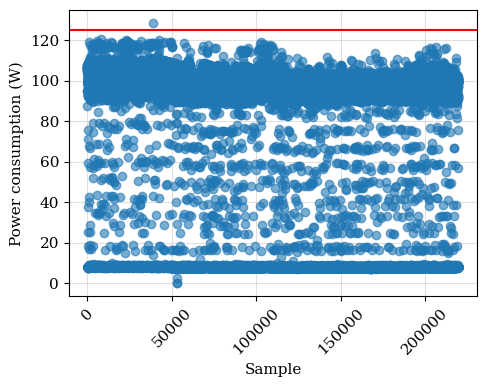
\includegraphics[width=.9\linewidth]{images/raw_consumptions/boiler.png}
    \caption{Boiler}
    \label{fig:boiler}
  \end{subfigure}
  \begin{subfigure}{\textwidth}
    \centering
    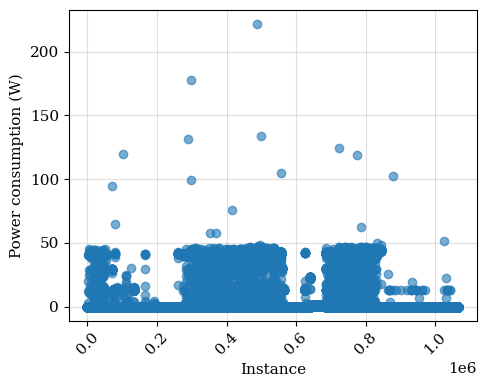
\includegraphics[width=.42\linewidth]{images/raw_consumptions/lamp.png}
    \caption{Lamp}
    \label{fig:lamp}
  \end{subfigure}
  \caption[Raw power consumptions of appliances extracted from UK-DALE]{Raw power consumptions of appliances extracted from UK-DALE. The samples are gathered every six seconds. The red line represents the maximum threshold used to clip the activations}
  \label{fig:raw_power_consumptions_uk_dale}
\end{figure}

\begin{table}
  \centering
  \resizebox{\textwidth}{!}{%
    \begin{tabular}{lccccc}
      \hline
      \textbf{Appliance type}                               &
      \multicolumn{1}{l}{\textbf{Min on (s)}}               &
      \multicolumn{1}{l}{\textbf{Min off (s)}}              &
      \multicolumn{1}{l}{\textbf{Activation Threshold (W)}} &
      \multicolumn{1}{l}{\textbf{Max Threshold (W)}}        &
      \multicolumn{1}{l}{\textbf{\# Activations}}                                           \\ \hline
      Radio                                                 & 5   & 5   & 10  & 100  & 1344 \\
      Dishwasher                                            & 90  & 90  & 30  & 400  & 727  \\
      Fridge w/ freezer                                     & 0   & 30  & 40  & 300  & 237  \\
      Television                                            & 20  & 20  & 10  & 175  & 239  \\
      Microwave                                             & 20  & 10  & 20  & 2200 & 2311 \\
      Lamp                                                  & 1   & 1   & 5   & 50   & 812  \\
      Washing machine                                       & 30  & 30  & 20  & 2200 & 609  \\
      Desktop                                               & 20  & 10  & 10  & 100  & 331  \\
      Boiler                                                & 10  & 5   & 50  & 125  & 607  \\
      AC                                                    & 120 & 120 & 300 & 1000 & 1095 \\ \hline
    \end{tabular}%
  }
  \caption{Parameters used to extract the activations for each appliance}
  \label{tab:activation_details}
\end{table}

\section{Autoencoder}

An autoencoder is a type of neural network capable of learning to compress the inputs into a low-dimensional representation, called the \textit{latent state}, in a totally unsupervised way~\parencite{hintonReducingDimensionalityData2006}. It has two components: an encoder that maps the inputs to the latent state, and a decoder that reconstructs the inputs from the latent state. The goal of the autoencoder is to learn the most relevant features of the inputs by minimizing the difference between the original and the reconstructed inputs, also known as the \textit{reconstruction error}~\parencite{hintonReducingDimensionalityData2006}. An autoencoder can learn the most important features of the activations of an appliance, so that they can be clustered to identify operation modes. Clustering the raw activations is not an effective approach, as it is too susceptible to noise~\parencite{castangiaClusteringApplianceOperation2023}, and requires extensive computational resources due to the high dimensionality of activations. The next sections describe the layers that make up the architecture used in this work.

\subsection{One-dimensional Convolutional Layers}

One-dimensional (1-D) convolutional layers are neural network layers commonly used to process sequential data, such as text, speech, audio, or time series. They learn temporal dependencies and meaningful features from the input data by applying 1-D convolutions~\parencite{kiranyaz1DConvolutionalNeural2021}. A convolution is a mathematical operation that slides a filter or \textit{kernel} over the input and computes the dot product between the filter and the input at each position~\parencite{rudinFunctionalAnalysisTata1973}. 1-D convolutional layers are composed of multiple filters that have the purpose of selecting the most salient features from the input sequence received from the previous layer. The greater the number of filters, the larger the amount of features that can be potentially learned~\parencite{castangiaClusteringApplianceOperation2023}. This is important to extract the most significant features of activations while removing noise. Each filter performs the computation in Equation~\eqref{equ:convolution}, where $n$ is the filter's size, $x_i$ are the inputs, $w_i$ are the filter's weights, $b$ is a bias term, and $f$ is the activation function.
\begin{equation}\label{equ:convolution}
  \tilde{y} = f(\sum_{i=1}^{n}{w_i x_i} + b)
\end{equation}

\newpage

Pooling and upsampling layers often accompany convolutional layers. Pooling layers shrink the output from the convolutional layer. Max pooling does this by taking the maximum value of a sliding window along the input sequence~\parencite{ahmadDeepLearningMultiscale2019}; this helps in selecting the most important features from the input, lower the computation and memory cost, and avoid overfitting~\parencite{zhangDiveDeepLearning2023,masciStackedConvolutionalAutoEncoders2011}. Upsampling layers are somewhat the opposite, as they enlarge their input by inserting zeros between the input values.

\subsection{Long-Short Term Memory}

\acrfull{lstm} is a type of \acrfull{rnn} that can learn long-term dependencies in sequential data. \acrshort{rnn}s are neural networks that have feedback loops, which allow them to process sequential data such as text, speech, audio, or time series~\parencite{ahmadDeepLearningMultiscale2019}. However, \acrshort{rnn}s often suffer from vanishing or exploding gradient, which makes it difficult to learn from distant past inputs or outputs. \acrshort{lstm} solves this problem by introducing a memory cell that can store, update, and retrieve information over long periods~\parencite{hochreiterLongShortTermMemory1997}. This is useful to learn both the short-term and long-term dependencies among the values of the activations of an appliance.

\acrshort{lstm}s use three gates (input, output, and forget) to control the information flow in and out of the memory cell. These gates can decide what information to keep or discard, based on the current input and the previous state. The full architecture is shown in Figure~\ref{fig:lstm_architecture}. At each time step, the \acrshort{lstm} cell takes the current input $X_t$ and a summary of all previous inputs, which is composed of the short-term state $H_{t-1}$ and the long-term state $C_{t-1}$. Equations~\eqref{equ:lstm_1}---\eqref{equ:lstm_6} show the different operations performed by the \acrshort{lstm} cell, where $W_{xi}$, $W_{xf}$, $W_{xo}$, and $W_{xc}$ are the weights of the input vector $X_t$; $W_{hi}$, $W_{hf}$, $W_{ho}$, and $W_{hc}$ are the weights of the previous short-term state vector $H_{t-1}$; $b_i$, $b_f$, $b_o$, and $b_c$ are the bias terms.
\begin{equation}\label{equ:lstm_1}
  I_t = \sigma(X_{t}W_{xi} + H_{t-1}W_{hi} + b_{i})
\end{equation}
\begin{equation}\label{equ:lstm_2}
  F_t = \sigma(X_{t}W_{xf} + H_{t-1}W_{hf} + b_{f})
\end{equation}
\begin{equation}\label{equ:lstm_4}
  O_t = \sigma(X_{t}W_{xo} + H_{t-1}W_{ho} + b_{o})
\end{equation}
\begin{equation}\label{equ:lstm_3}
  \tilde{C}_t = \tanh(X_{t}W_{xc} + H_{t-1}W_{hc} + b_{c})
\end{equation}
\begin{equation}\label{equ:lstm_5}
  C_t = F_t \odot C_{t-1} + I_t \odot \tilde{C}_t
\end{equation}
\begin{equation}\label{equ:lstm_6}
  H_t = O_t \odot \tanh(C_t)
\end{equation}

\begin{figure}
  \centering
  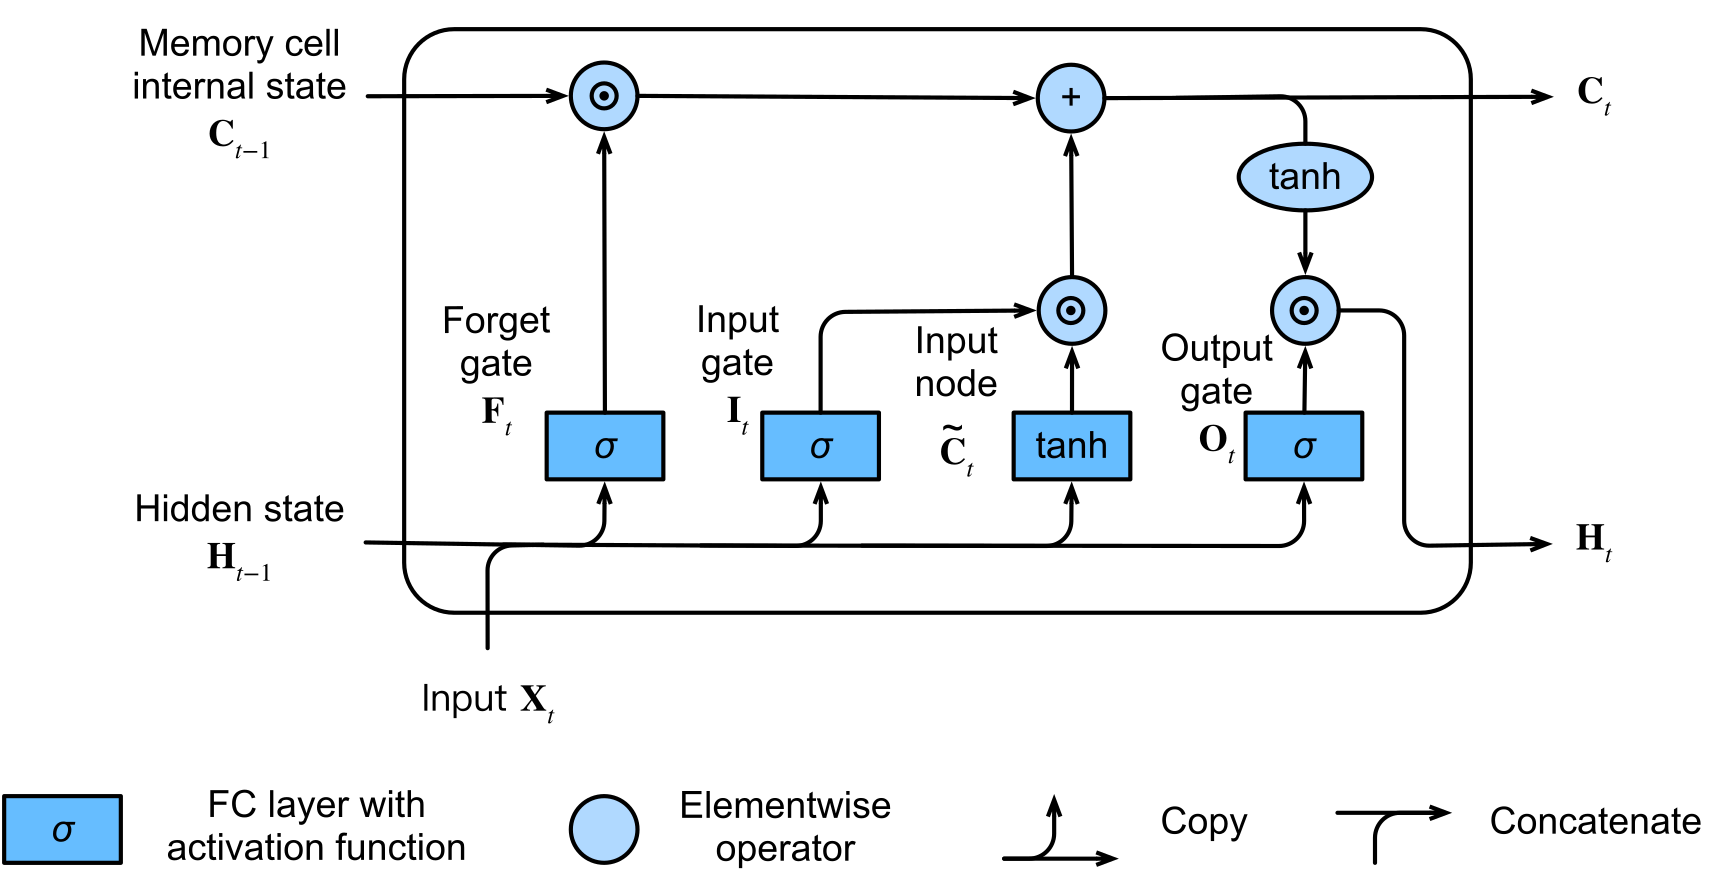
\includegraphics[width=.65\linewidth]{images/modes_clustering/lstm.png}
  \caption[LSTM cell architecture]{LSTM cell architecture. From~\textcite{zhangDiveDeepLearning2023}, Subsection 10.1.1, CC-BY-SA 4.0 license}
  \label{fig:lstm_architecture}
\end{figure}

A \acrfull{bilstm} is a combination of two \acrshort{lstm}s that process the input sequence in both forward and backward directions~\parencite{schusterBidirectionalRecurrentNeural1997}. One \acrshort{lstm} takes the input sequence as it is, and the other \acrshort{lstm} takes the input sequence in reverse order. The outputs of both \acrshort{lstm}s are then concatenated or summed to produce the final output. A \acrshort{bilstm} can capture both the past and future context of the input sequence and learn which direction is more important for each output step.

\subsection{Autoencoder Architecture and Training}

Figure~\ref{fig:autoencoder_architecture} shows the autoencoder architecture used. The encoder has six convolutional layers with max-pooling layers in between, which halve their input dimensions. It ends with two \acrshort{lstm} layers that capture temporal relations among activation values. The first \acrshort{lstm} layer is bidirectional, and the second is unidirectional. The decoder begins with a repeat vector layer to replicate the latent state six times, to reconstruct the correct output dimensions. It then continues with an \acrshort{lstm} layer followed by a series of convolutions and up-sampling layers that double their input dimensions. All convolutional layers have $32$ filters of size $3$, with a \acrfull{relu} activation function. To keep the same sequence length after the convolution, the stride is $1$ and zero padding is added to the input sequence on both sides. The \acrshort{lstm} cells have $128$ units and use a hyperbolic tangent (tanh) activation function.

\begin{figure}
  \centering
  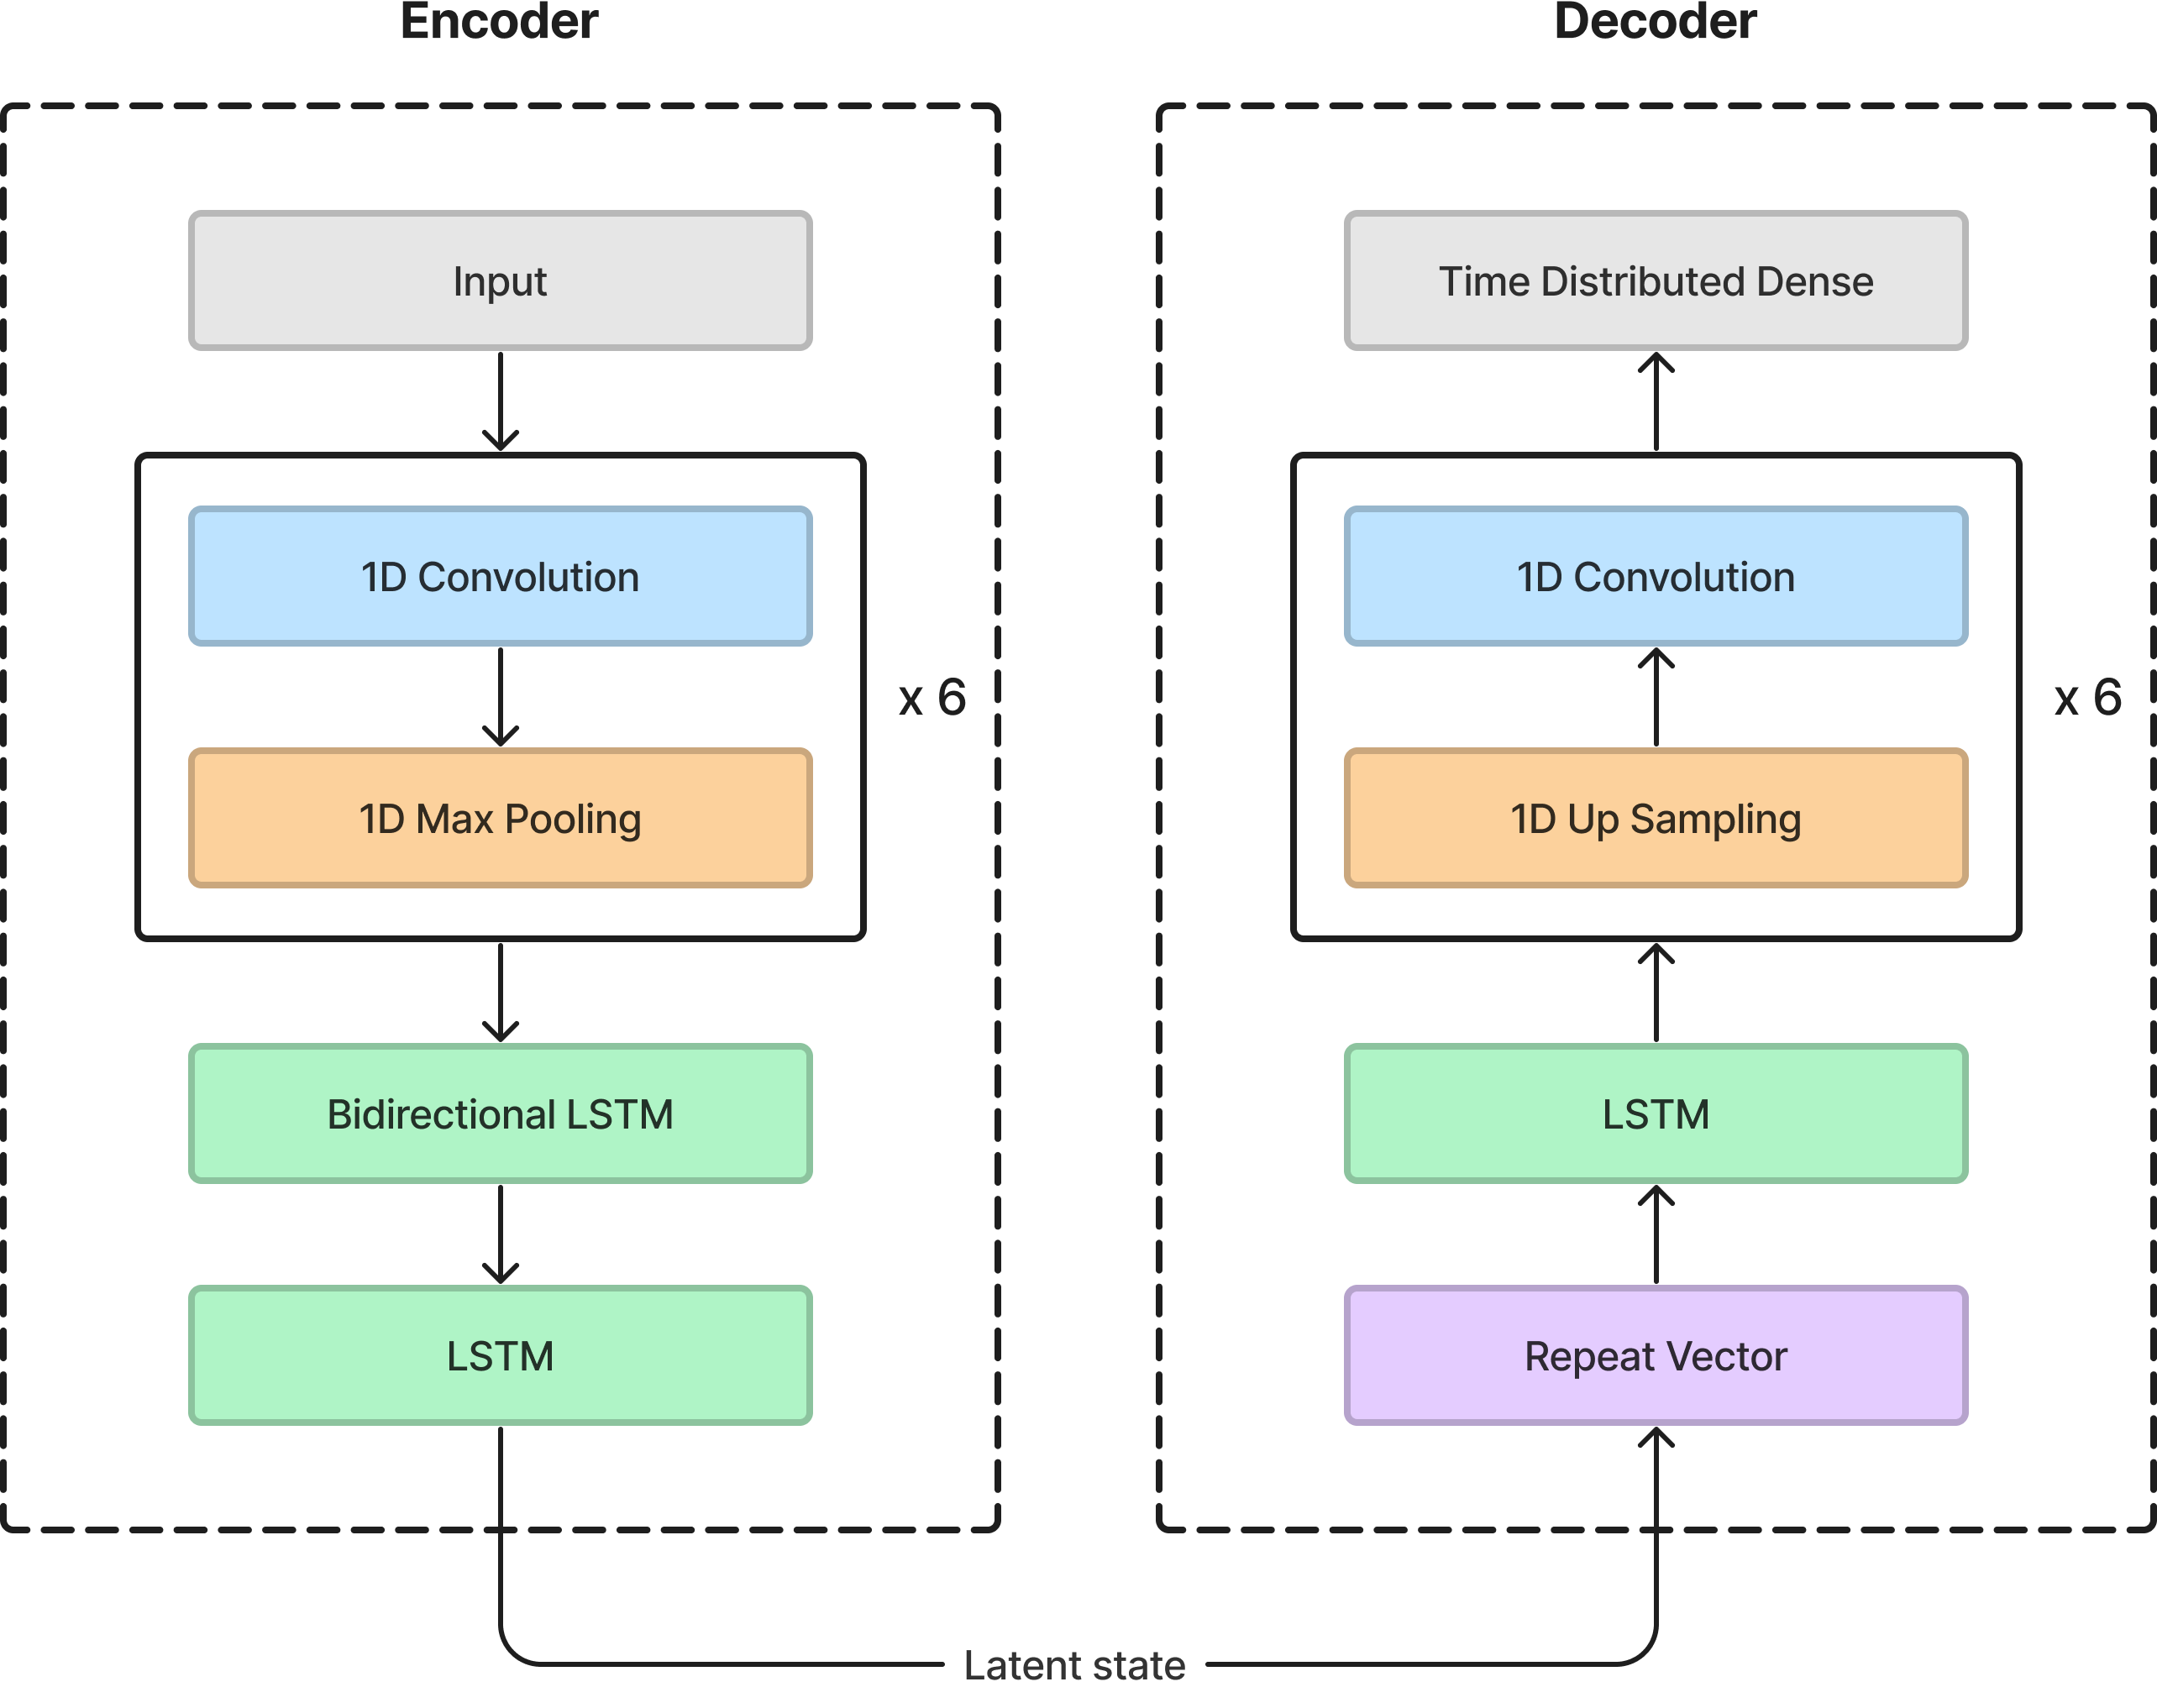
\includegraphics[width=.8\linewidth]{images/modes_clustering/autoencoder.png}
  \caption{Architecture of the autoencoder}
  \label{fig:autoencoder_architecture}
\end{figure}

The model was implemented using Tensorflow~\parencite{abadiTensorFlowLargeScaleMachine2016,tensorflowdevelopersTensorFlow2023} version \texttt{2.15.0} and Keras~\parencite{cholletKeras2015}, in the version provided by Tensorflow. The Python version is \texttt{3.10.12}. The training was executed using a Google Colab notebook\footnote{\url{https://colab.research.google.com/drive/1blnoyyP10gGdRL6b4JzaeBLg8zs2kVv9?usp=sharing}}, running \texttt{Ubuntu 22.04.03 LTS} with the Linux kernel \texttt{6.1.58}, with an \texttt{Intel Xeon 2.00GHz} CPU, a \texttt{Tesla T4} GPU, and $12.6GB$ of RAM.

The loss function used is the mean square error between the output and the original input. The network parameters are optimized by using the \acrfull{adam} algorithm with a learning rate of $0.001$ and a batch size of $32$. The training process lasts for $500$ epochs at most, but it stops sooner if the loss value does not improve for $40$ epochs, returning the best model found. The $20\%$ of training instances were held out for training validation. All training instances are zero-padded or truncated to $896$ samples. This number was chosen as it is close to the average length of all activations, and it is divisible by $2$ for $6$ times, which ensures that the up-sampling layers in the decoder correctly reconstruct the input dimensions. The instances are then standardized using Equation~\eqref{equ:std}, where the mean $\mu_X$ and standard deviation $\sigma_X$ are computed across all the power measurements $X$. The evolution of the training and validation loss values during training are reported in Figure~\ref{fig:autoencoder_losses}.
\begin{equation}\label{equ:std}
  X_{scaled} = \frac{X - \mu_X}{\sigma_X}
\end{equation}

\begin{figure}
  \centering
  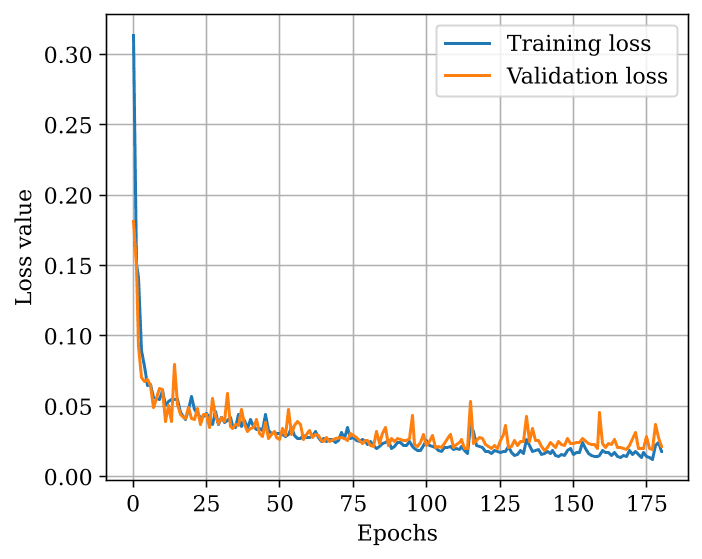
\includegraphics[width=.6\linewidth]{images/modes_clustering/loss.png}
  \caption{Evolution of training and validation losses during training}
  \label{fig:autoencoder_losses}
\end{figure}

\section{Modes Clustering}

The complete clustering procedure for the operation modes of appliances is illustrated in Figure~\ref{fig:clustering}. First, the activations of each appliance are standardized using Equation~\eqref{equ:std}. Then, the latent state of each activation is obtained by applying the trained encoder. Next, the K-Means algorithm is used to cluster the latent states into $K$ groups. The algorithm iteratively assigns each latent state to the closest cluster centroid, calculated as the mean of all instances in a cluster, thus minimizing the mean squared distance between the instances and their centroids~\parencite{lloydLeastSquaresQuantization1982}. The algorithm converges when the centroids stop changing. The scikit-learn~\parencite*{pedregosaScikitlearnMachineLearning2011, buitinckAPIDesignMachine2013} implementation of K-Means was used, with the default settings that select a single initial centroid chosen by the \textit{k-means++} method, based on the points’ inertia. The algorithm also has a maximum of $300$ iterations and a tolerance of $0.0001$.

\begin{figure}
  \centering
  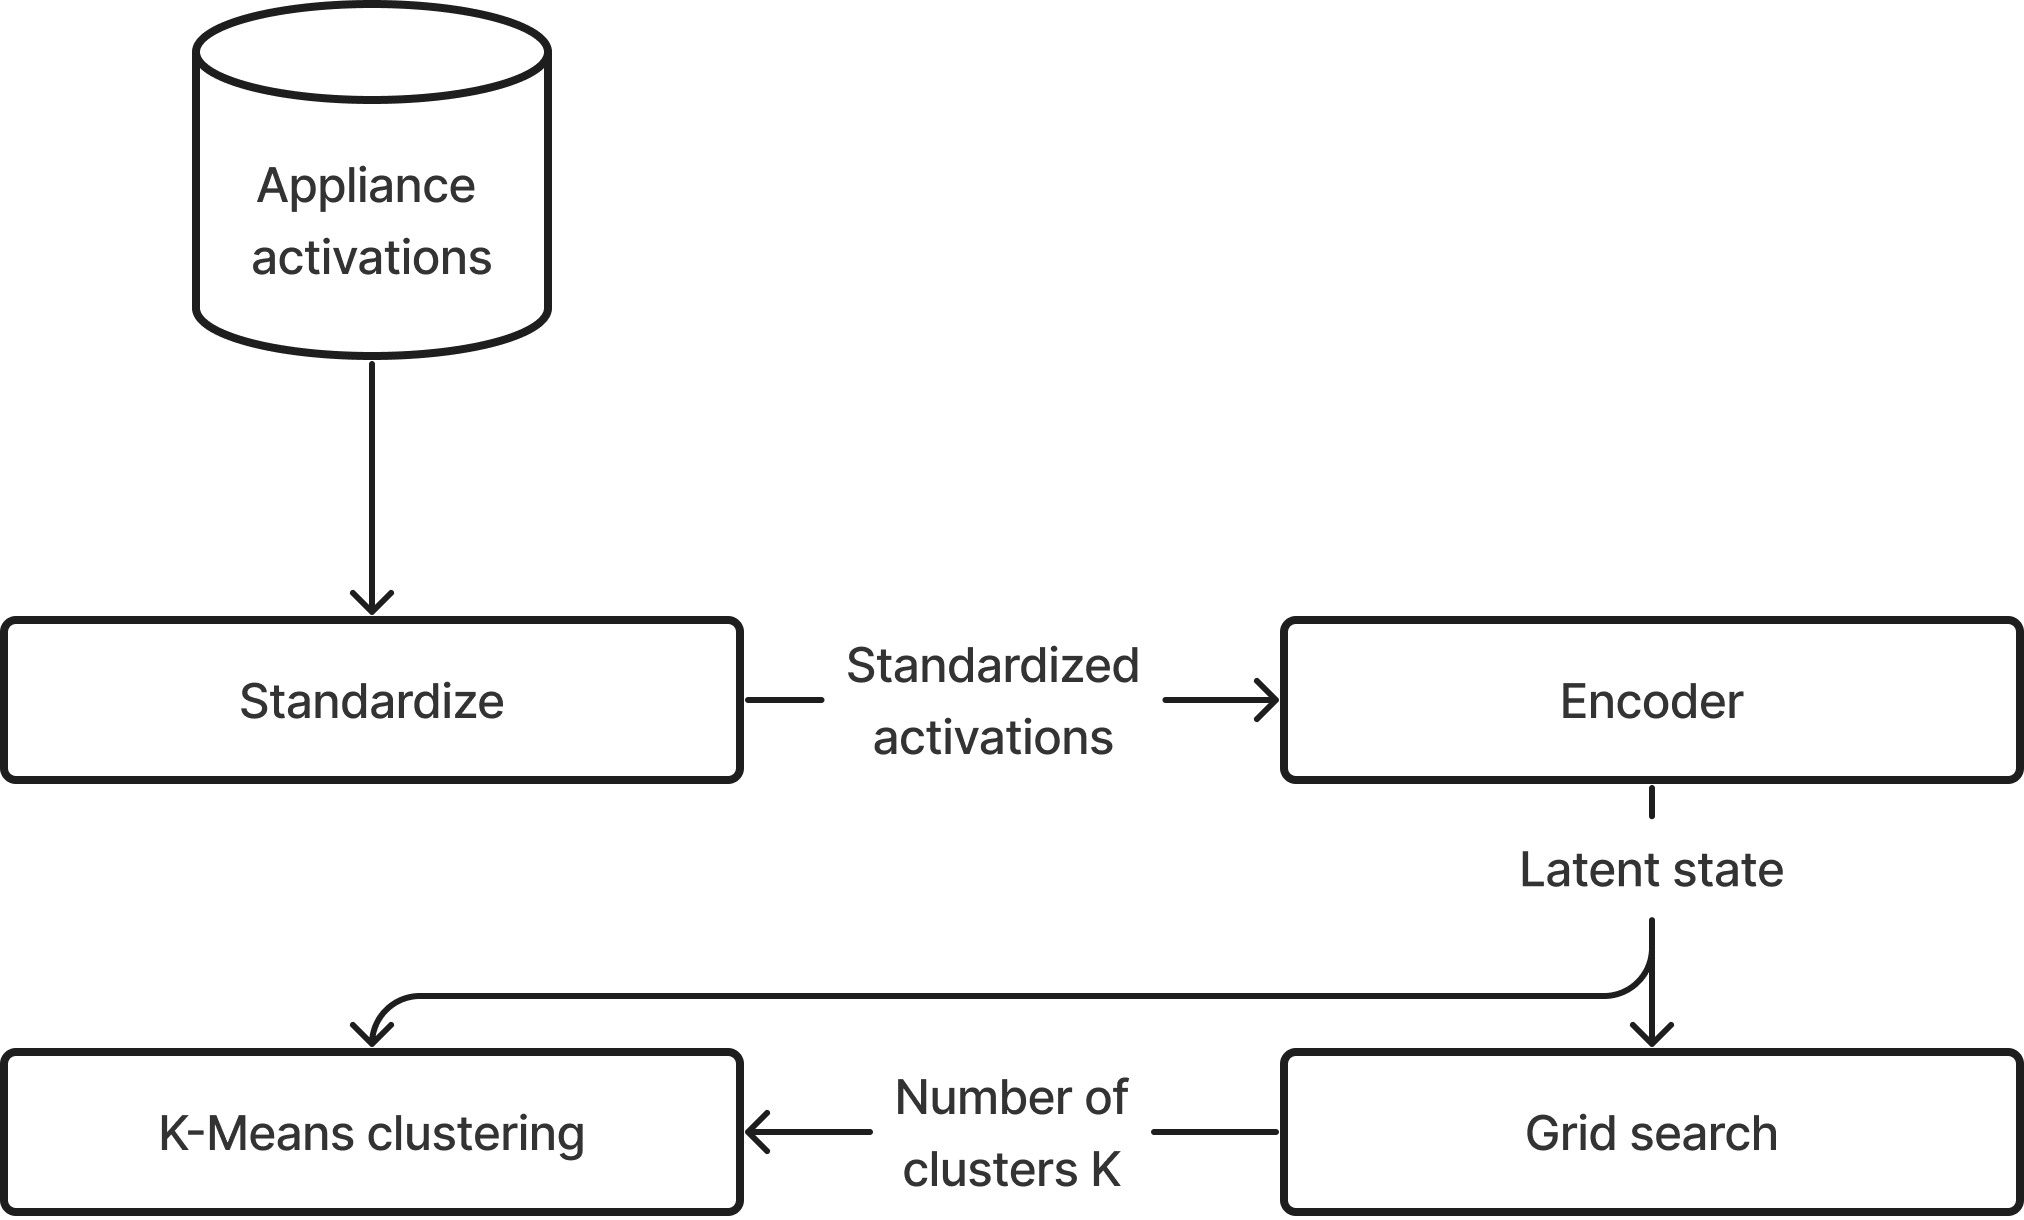
\includegraphics[width=.5\linewidth]{images/modes_clustering/clustering.png}
  \caption{Procedure for clustering the operation modes of appliances}
  \label{fig:clustering}
\end{figure}

To find the optimal number of clusters K for each appliance, a grid search was run to evaluate the \textit{silhouette score} of each possible clustering. The silhouette score quantifies how well a latent state belongs to its cluster compared to other clusters~\parencite{rousseeuwSilhouettesGraphicalAid1987}. It is computed for each latent state using Equation~\eqref{equ:silhouette}, where $a(i)$ is the mean squared distance between the latent state and the other latent states in the same cluster, and $b(i)$ is the minimum mean squared distance between the latent state and the latent states in different clusters. The silhouette score ranges from $-1$ to $1$, with higher values indicating better clustering. The average silhouette score of all the latent states is used as a metric for the quality of the clustering as a whole.
\begin{equation}\label{equ:silhouette}
  s(i) = \frac{b(i) - a(i)}{\max{a(i), b(i)}}
\end{equation}

The clustering with the highest silhouette score was chosen. The search space for K was limited to values between $2$ and $4$, because lower values would not capture the diversity of the operation modes, and higher values would create too many noise clusters that could not be interpreted as meaningful modes. This also matches the realistic expectation that end users do not make use of all the operation modes for their appliances. For instance, it is possible that an end user only uses a washing machine with a few programs, such as a quick wash or a delicate wash, and never uses the other programs.

\section{Identification of Operation Modes}

The cluster labels were used to identify the operation modes of the appliance and to estimate their duration. The procedure used for doing this is presented in Figure~\ref{fig:identification}.

\begin{figure}
  \centering
  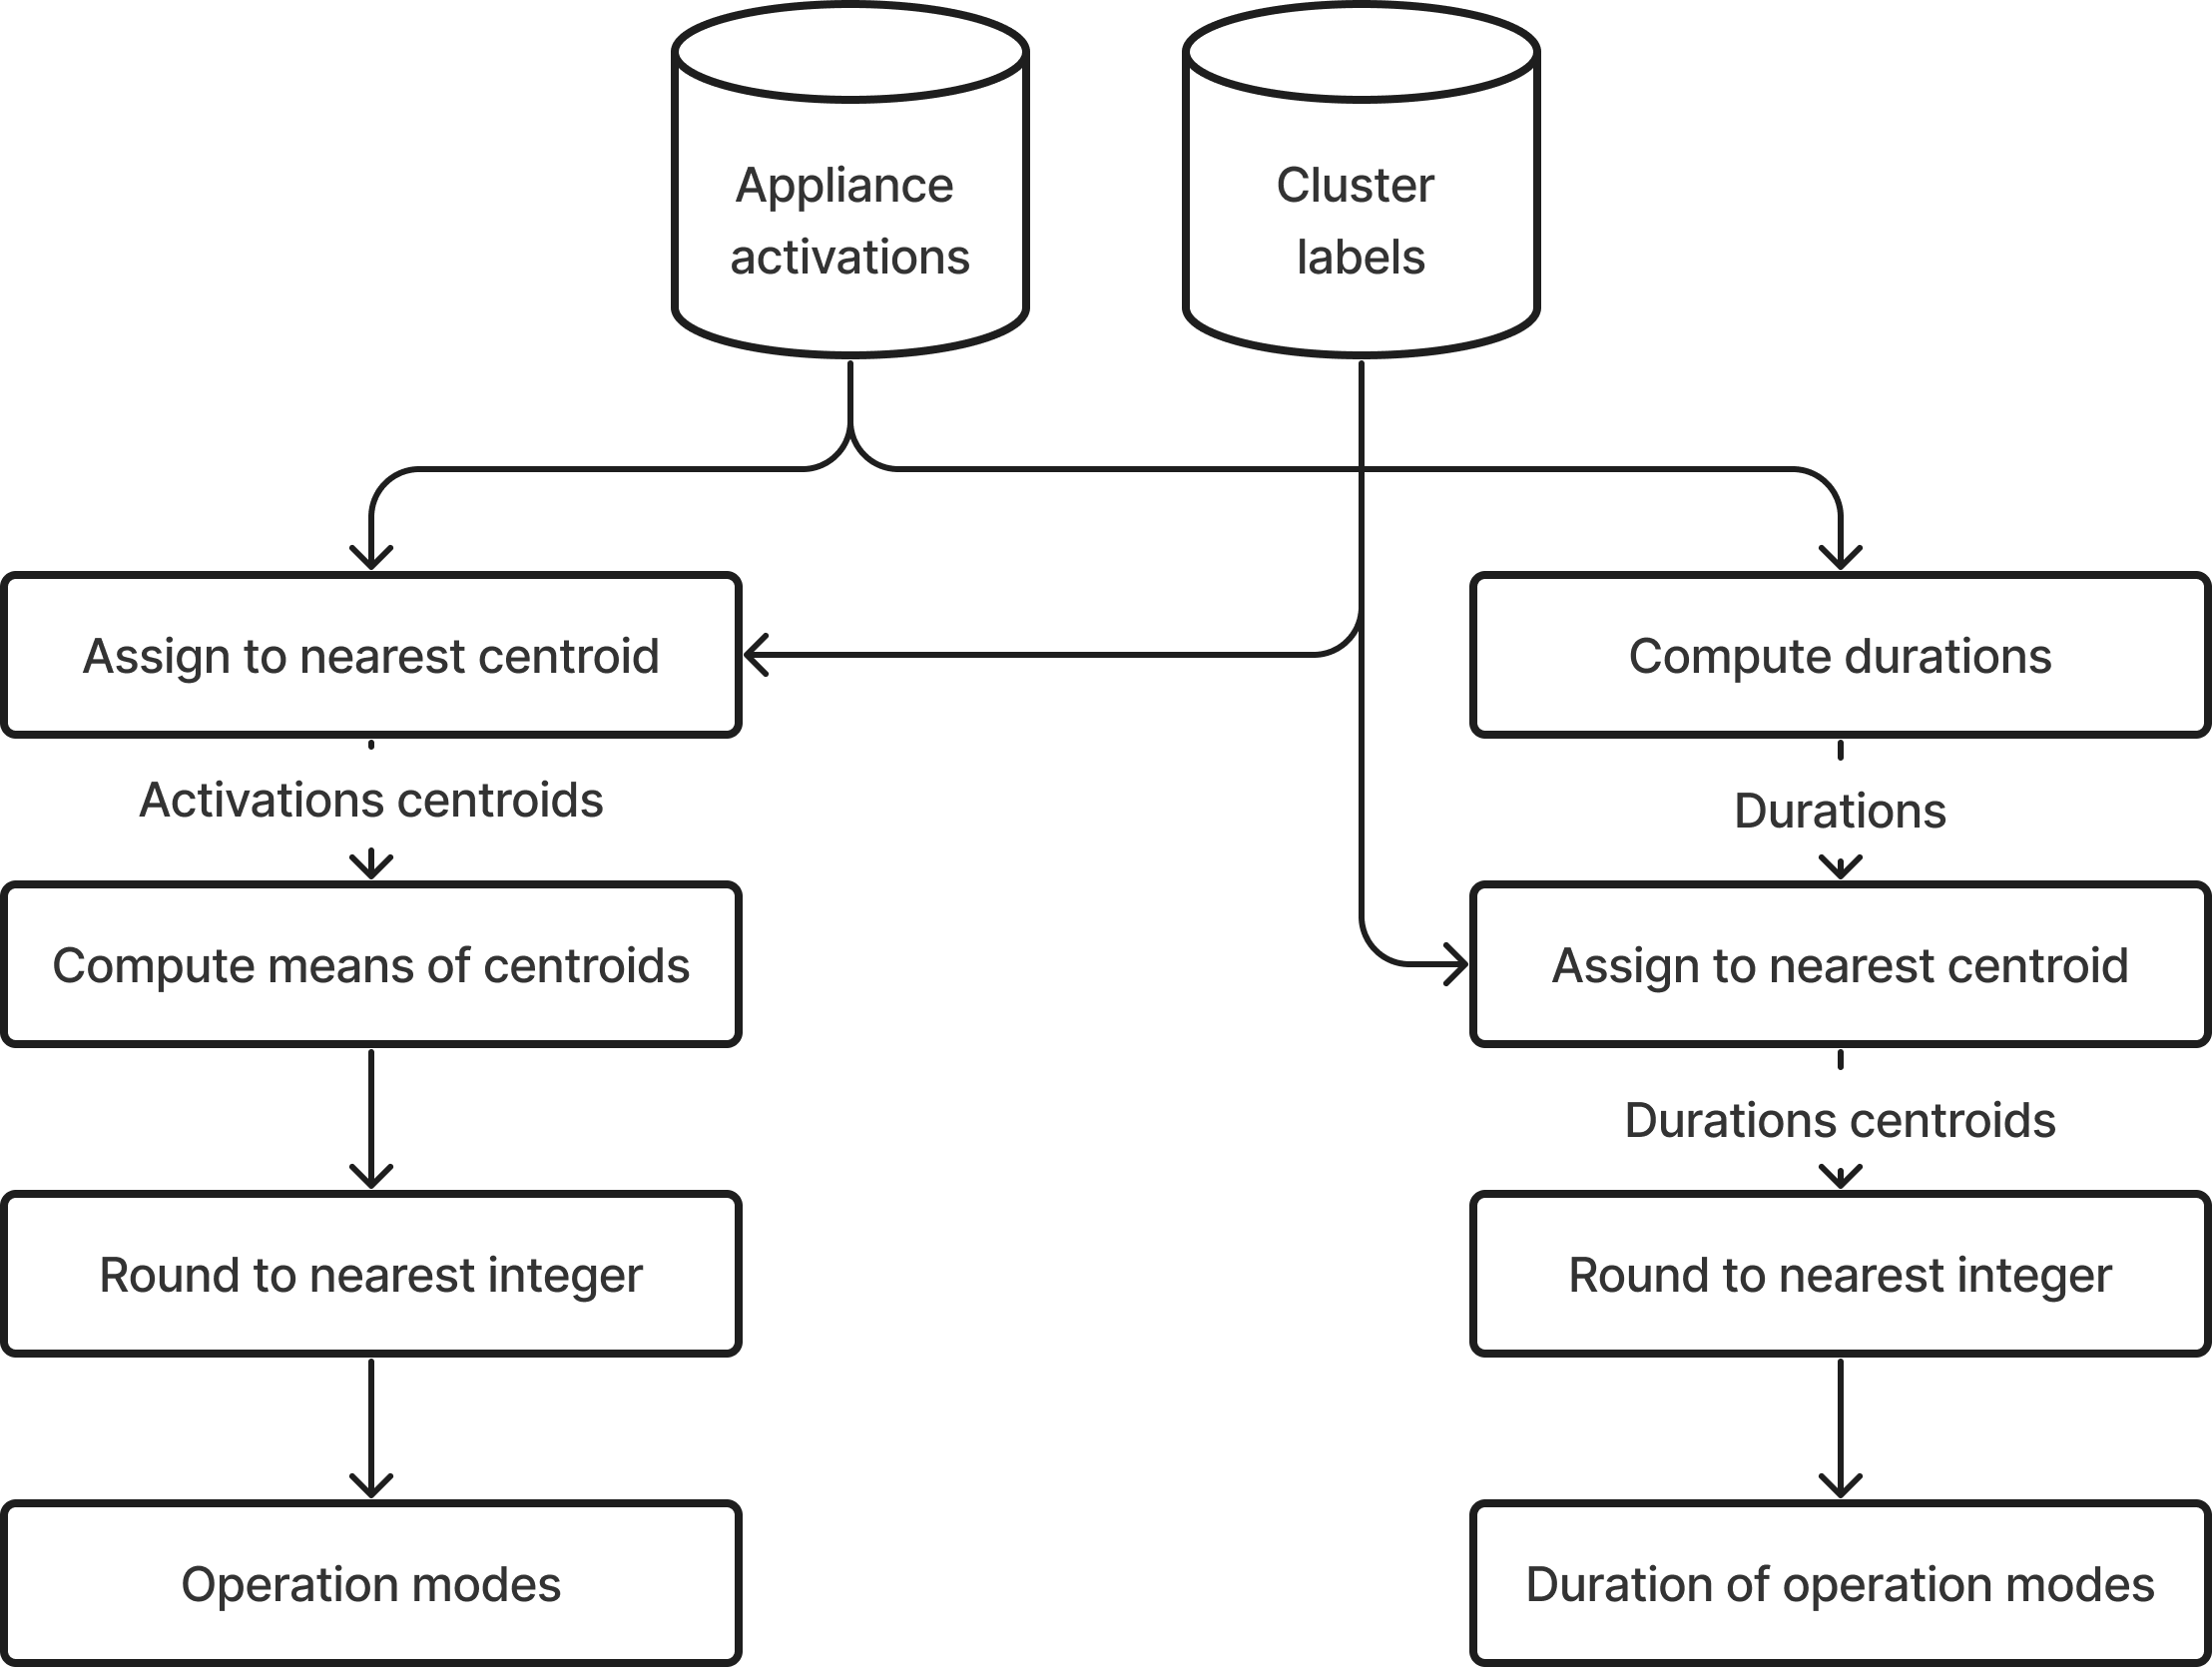
\includegraphics[width=.55\linewidth]{images/modes_clustering/identification.png}
  \caption{Procedure for identifying the operation modes of appliances}
  \label{fig:identification}
\end{figure}

First, the appliance activations are assigned to the closest cluster centroid, which represents the mean activation of each cluster. Then, the mean power consumption value of each centroid is computed and rounded to the nearest integer. These values are the potential operation modes of the appliance. Next, a selection process is performed to merge or discard operation modes that have similar or unrealistic power consumption values, based on the device manuals. The manuals also provide the names of the identified modes. This procedure may not detect all the operation modes, especially if the end users do not use some of them frequently, or if the procedure confuses transitional states with modes.

Second, the duration of each operation mode is estimated by calculating the average duration (in seconds) of the activations that belong to the same cluster. The duration values are also rounded to the nearest integer. These values are used as default durations for the operation modes. The obtained preliminary results are reported in Table~\ref{tab:preliminary_identification_results}.

\begin{table}[hbt]
  \centering
  \resizebox{.39\textwidth}{!}{%
    \begin{tblr}{lcc}
      \hline
      \textbf{Appliance type}             & \textbf{Consumption (W)} & \textbf{Duration (s)} \\ \hline
      \SetCell[r=2]{l}{Radio}             & 1                        & 80                    \\
                                          & 37                       & 4435                  \\ \hline[dashed]
      \SetCell[r=4]{l}{Dishwasher}        & 136                      & 2359                  \\
                                          & 12                       & 240                   \\
                                          & 54                       & 3025                  \\
                                          & 41                       & 459                   \\ \hline[dashed]
      \SetCell[r=2]{l}{Fridge w/ freezer} & 208                      & 6304                  \\
                                          & 7                        & 37                    \\ \hline[dashed]
      \SetCell[r=2]{l}{Television}        & 18                       & 2514                  \\
                                          & 110                      & 1833                  \\ \hline[dashed]
      \SetCell[r=2]{l}{Microwave}         & 42                       & 302                   \\
                                          & 1265                     & 1433                  \\ \hline[dashed]
      \SetCell[r=2]{l}{Lamp}              & 2                        & 309                   \\
                                          & 19                       & 587                   \\ \hline[dashed]
      \SetCell[r=4]{l}{Washing machine}   & 82                       & 1176                  \\
                                          & 118                      & 1486                  \\
                                          & 1281                     & 1309                  \\
                                          & 1783                     & 1511                  \\ \hline[dashed]
      \SetCell[r=2]{l}{Desktop}           & 4                        & 1159                  \\
                                          & 41                       & 12412                 \\ \hline[dashed]
      \SetCell[r=3]{l}{Boiler}            & 33                       & 300                   \\
                                          & 57                       & 525                   \\
                                          & 101                      & 2187                  \\ \hline[dashed]
      \SetCell[r=3]{l}{AC}                & 71                       & 199                   \\
                                          & 336                      & 3337                  \\
                                          & 656                      & 30176                 \\ \hline
    \end{tblr}%
  }
  \caption[Preliminary results of operation modes identification]{Preliminary results of operation modes identification. The \textit{off} mode is not reported, as it is assumed to have 0W consumption and indeterminate duration for all appliances}
  \label{tab:preliminary_identification_results}
\end{table}

The procedure works well for simple appliances, such as the lamp or the television, whose operation modes are easy to distinguish. However, it has some limitations for more complex appliances, such as the washing machine, the dishwasher, and the microwave. For these appliances, the procedure fails to identify the correct operation modes and their durations, due to the following reasons:
\begin{itemize}
  \item The sequence length of $896$ is too short to capture the full cycle of these appliances, which may have multiple operation modes in one activation.
  \item The number of training instances for the autoencoder is too small to learn the features of these appliances, which may have high variability in their activations.
  \item The extraction of the activations is based on an empirical threshold, which may not be optimal for these appliances, whose power consumption may fluctuate or overlap with other appliances.
  \item The operation modes are too similar to each other, or there are too many to be distinguishable. This could be the case with the microwave, which allows the user to manually configure the power level of each operation mode, thus creating a large number of possibilities.
\end{itemize}

Therefore, for the washing machine, dishwasher, and microwave, the operation modes and their durations were extracted from the manuals of the devices. For appliances with configurable operation modes, only a single configuration was chosen to represent each mode. The identified durations for \textit{stand-by} or \textit{suspended} operation modes were set to $\infty$, as such modes typically remain active until the user explicitly changes them. Table~\ref{tab:identification_results} summarizes the results of the identification procedure for all the appliances.

\begin{table}
  \centering
  \resizebox{.6\textwidth}{!}{%
    \begin{tblr}{llcc}
      \hline
      \textbf{Appliance type}           & \textbf{Mode name} & \textbf{Consumption (W)} & \textbf{Duration (s)} \\ \hline
      \SetCell[r=2]{l}{Radio}           & Stand-by           & 1                        & $\infty$              \\
                                        & On                 & 37                       & 4435                  \\ \hline[dashed]
      \SetCell[r=6]{l}{Dishwasher}      & Intensive          & 1400                     & 10380                 \\
                                        & Daily              & 810                      & 10260                 \\
                                        & Eco                & 700                      & 6660                  \\
                                        & Express            & 350                      & 1680                  \\
                                        & Delicate           & 800                      & 7080                  \\
                                        & Pre-wash           & 10                       & 660                   \\ \hline[dashed]
      Fridge w/ freezer                 & On                 & 208                      & 6304                  \\ \hline[dashed]
      \SetCell[r=2]{l}{Television}      & Stand-by           & 18                       & 2514                  \\
                                        & On                 & 110                      & 1833                  \\ \hline[dashed]
      \SetCell[r=7]{l}{Microwave}       & Stand-by           & 5                        & $\infty$              \\
                                        & Microwave          & 750                      & 300                   \\
                                        & Crisp              & 500                      & 300                   \\
                                        & Grill              & 500                      & 300                   \\
                                        & Grill+microwave    & 500                      & 300                   \\
                                        & Steam              & 350                      & 300                   \\
                                        & Jet defrost        & 160                      & 300                   \\ \hline[dashed]
      Lamp                              & On                 & 19                       & 587                   \\ \hline[dashed]
      \SetCell[r=7]{l}{Washing machine} & Cotton 90°         & 2000                     & 8700                  \\
                                        & Cotton 60E         & 950                      & 7680                  \\
                                        & Cotton 60°         & 1200                     & 7200                  \\
                                        & Cotton 30°         & 550                      & 6900                  \\
                                        & Synthetic 30°      & 900                      & 5400                  \\
                                        & Delicate 30°       & 500                      & 3600                  \\
                                        & Wool               & 450                      & 3300                  \\ \hline[dashed]
      \SetCell[r=2]{l}{Desktop}         & Suspended          & 4                        & $\infty$              \\
                                        & On                 & 41                       & 12412                 \\ \hline[dashed]
      \SetCell[r=3]{l}{Boiler}          & Holiday            & 33                       & 300                   \\
                                        & Comfort            & 57                       & 525                   \\
                                        & Auto               & 101                      & 2187                  \\ \hline[dashed]
      \SetCell[r=2]{l}{AC}              & Cool               & 336                      & 3337                  \\
                                        & Heat               & 656                      & 30176                 \\ \hline
    \end{tblr}%
  }
  \caption[Results of operation modes identification]{Results of operation modes identification. The \textit{off} mode is not reported, as it is assumed to have 0W consumption and indeterminate duration for all appliances}
  \label{tab:identification_results}
\end{table}

    \chapter{Digital Twin}\label{ch:digital_twin}

\begin{lstlisting}[language=json,caption={JSON file describing the fridge.},label=fridge_json,float,floatplacement=H]
{
    "id": 4,
    "device": "fridge freezer",
    "manufacturer": "Siemens",
    "model": "",
    "location": "kitchen",
    "modes": [
        {
            "id": 0,
            "name": "off",
            "power_consumption": 0
        },
        {
            "id": 1,
            "name": "on",
            "power_consumption": 208
        }
    ]
}
\end{lstlisting}
    \chapter{Conclusions and Future Work}\label{ch:conclusions}

This thesis presents a \acrshort{dt} for smart homes that can forecast and optimize the energy consumption of various appliances in a smart home. A hypothetical home was used as a case study to design and test the \acrshort{dt}, since no real home was available. The hypothetical home included a range of appliances that were representative of typical smart home scenarios.

A scoping review of existing smart home datasets was performed to select suitable data sources for the appliances. The review revealed that power consumption datasets were the most relevant and available, but none of them contained information about the operation modes of the appliances. To address this limitation, 15 appliances from the GREEND and UK-DALE datasets were chosen, and their operation modes were inferred using a hybrid \acrshort{ml} method and the manufacturers' manuals.

The \acrshort{dt} was implemented as a \acrshort{rest} \acrshort{api}, which offers several endpoints to access and manipulate information about appliances, routines, and consumptions. The \acrshort{api} also allows to simulate the addition of new routines and provides feedback and suggestions to improve energy efficiency. A frontend application was developed to showcase the functionality and usability of the \acrshort{dt}.

\paragraph{Physical Twin}

The \acrshort{dt} developed in this thesis is a digital-only system that cannot interact with the physical world directly. To enable this interaction, it needs to connect to the smart devices in the home and send commands to them. This entails developing a physical twin similar to the hypothetical home presented in Chapter~\ref{ch:hypothetical_home}. The \acrshort{dt} should also update the state of the devices and the energy consumption according to the changes in the physical world.

\paragraph{Appliance Data}

Future versions of the \acrshort{dt} should let users add new appliances by automatically importing their consumption values and operation modes. This requires having a list of smart devices that are compatible with the \acrshort{dt}, and whose data are accessible during the system configuration. Since the appliance data format is custom, it may be necessary to use a standardized format for the data or develop a system that can automatically convert the data from the appliance to the format used by the \acrshort{dt}.

These consumption values should be treated as approximate and based on the new and optimal functioning of the appliance. Over time, the \acrshort{dt} should learn from the actual consumption, as they may vary due to malfunctions or lack of maintenance.

The \acrshort{dt} could also work with non-smart appliances that do not provide information about themselves, by using a \acrshort{ml} approach similar to the one used in Chapter~\ref{ch:hypothetical_home} to automatically detect the operation modes and consumptions.

\paragraph{Manual Appliance Activation}

The \acrshort{dt} should be able to handle the manual activation of appliances by end users, by automatically detecting their state changes and resolving conflict C3 (see Section~\ref{sec:simulation}).

Moreover, the \acrshort{dt} could monitor the manual activations of appliances and their duration, and use this information to provide suitable recommendations to automate the activations or modify existing routines. For instance, if the user starts the computer every day at 9:00, the \acrshort{dt} could propose to automate this activation. If the computer stays on for 8 hours on average, the \acrshort{dt} can use this information to anticipate whether this could cause any conflict with existing routines, and avoid them before they occur.

\paragraph{Predictions over Multiple Days}

Currently, the \acrshort{dt} can only predict the energy consumption for the current day. Future versions should enable the system to predict the energy consumption for several days ahead, and also view the consumption history for the previous days. This would allow the system to provide more precise recommendations, and to better handle the conflicts between routines. For example, if the user is planning to go on vacation for a week, the \acrshort{dt} could advise to turn off the heating system, and to turn off the refrigerator for the vacation period.

\paragraph{Authentication}

Future developments should implement an authentication scheme to secure the \acrshort{dt} from unauthorized access. This would enable the system to be used in a multi-user environment, where users may have different roles and permissions. This could be beneficial for a family, where the children are restricted from changing routines, and have limited access to creating new ones. For instance, they may be prohibited from creating routines that involve the dishwasher or the washing machine, and they may only activate the TV for a certain amount of time. The parents, on the other hand, may have full access to the system and could also monitor the children's activities.

\paragraph{Frontend}

To allow the end users to interact with the \acrshort{dt} effectively and also consider the future developments mentioned in the previous sections, a more comprehensive frontend application than the showcase one developed in this thesis is required. A frontend application for Android devices that meets these requirements is currently being developed as part of the broader research project.

\vspace*{\fill} % Spazio bianco per mettere il testo in fondo alla pagina

\begin{figure}[h]
    \centering
    
\includegraphics[width=.7\textwidth]{images/signature.png}
\end{figure}

\vspace*{16mm} % Spazio bianco per mettere il testo in fondo alla pagina
    
    \printbibliography[heading=bibintoc] % Bibliografia nell'indice
    
    \chapter*{Acknowledgments}\label{ch:acknowledgments}
\addcontentsline{toc}{chapter}{Acknowledgments}

I would like to express my deepest appreciation to Prof.\ Barbara Rita Barricelli and Prof.\ Daniela Fogli for their invaluable guidance and support throughout my thesis. They have been patient, encouraging, and knowledgeable mentors who have inspired me to pursue excellence. I also appreciate the support and resources provided by the entire staff of the University of Brescia, which enabled me to complete this thesis successfully.

This journey would not have been possible without the support of my parents, who have sacrificed so much to give me the opportunity to follow my dreams. I hope to make you proud.

I owe a huge debt of gratitude to the special people in my life who have always stood by me. Linda, you have always been a source of joy and strength for me, and I cannot thank you enough for bearing with me during the most difficult times. I hope you'll let me annoy you for a long time to come. Alessia, Federica, and Samuele, you have been amazing travel companions and friends, and I cherish your support and encouragement across the distance that separates us. Lara, you have been a loyal and caring friend who has always helped me in times of need. Daniela, Davide, Simone, and Stefano, you have been a constant and reliable presence in these uncertain years.

Finally, I cannot forget the Collegio Lucchini, where I have spent the last seven years of my life. It has offered me incredible opportunities, experiences, and friendships that I will always treasure. I am thankful to all the people who have shared this journey with me, both the “old guard” and the newcomers. Naming them all is not easy, but I will try: Alberto, Alessandra, Alessandro, Alice, Annabell, Antonio, Barak, Bruno, Camilla, Chiara, Daniele, Dumy, Filippo, Gaia, Giada, Giaele, Giulia, Ilenia, Jozef, Marcos, Martina, Matteo, Michele Fioroni, Michele Morselli, Nicholas, Wade. I also want to recognize the staff of the Collegio: Andrea Galli, Carla Bisleri, Laila Bellini, Lorenzo Gafforini, Luigi Negretti, Marta Perrini, and Paolo Carli. Thanks also to Beatrice Faedi, who introduced me to the world of theater. You have all contributed in making this place my home, and it is not going to be easy to leave.


\end{document}